\chapter{Applications}
\label{chapter:applications}

This chapter demonstrates the applicability of our method. First, we list practical examples of \PBN{} control in the field of regenerative medicine (cell reprogramming). We show the way the cell programming can be achieved on a specific example of a myeloid cell. Then we explain a holistic workflow of how the control of partially specified Boolean networks can be used to design a therapy or to refine the model. Finally, we show the full workflow on the second case study that is focused on the MAPK signalling pathway and demonstrates the control-guided model refinement.

\section{Motivation: cell reprogramming}
\label{sec:cell_reprogramming}

In nature, the most common process by which a cell acquires a different phenotype is \emph{cell differentiation}. A typical example is the differentiation of stem cells into specialised daughter cells in response to the organism's needs. The outcome of this process is often described as a \emph{cell fate} (or a cell-fate decision). Another natural mechanism is \emph{cell dedifferentiation} (or \emph{retrodifferentiation}), in which differentiated cells revert to an earlier developmental state. Dedifferentiation is observed in certain organisms, such as worms and amphibians~\cite{Jopling2011}. In addition, under specific conditions, differentiated cells can convert directly into a different differentiated cell type; this process is known as \emph{transdifferentiation}. These processes are illustrated in \autoref{fig:transdifferentiation}. The existence of such natural mechanisms has provided important inspiration for the emerging field of \emph{regenerative medicine}.

\begin{figure}
  \centering
  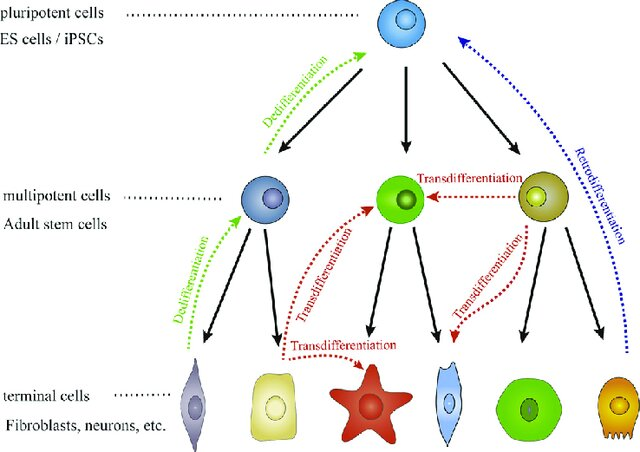
\includegraphics[width=0.65\textwidth]{Figures/transdifferentiation.jpg}
  \caption{\textbf{Cell differentiation.} From~\cite{Wang2012}. The figure illustrates examples of, and differences among, cell differentiation, dedifferentiation, and transdifferentiation.}
  \label{fig:transdifferentiation}
\end{figure}

The organism's need for cell differentiation is communicated via \emph{signalling pathways}~\cite{bradshaw2010}. These signals are transmitted via cascades of biochemical reactions, predominantly through protein phosphorylation catalyzed by protein kinases. Such signalling dynamics can be modelled using Boolean networks. If we can identify the signals that promote dedifferentiation or transdifferentiation, we may be able to emulate them and artificially induce the corresponding cellular transition. This procedure is known as \emph{cell reprogramming}. In this context, finding efficient perturbations for controlling BNs provides an abstract formulation of the signal-identification problem.

\emph{T-cells} are a central component of the human immune system. They must differentiate rapidly to mount an effective immune response. However, diseases affecting the  immune or haematopoietic system (e.g., leukaemia) can disrupt the signalling pathways that regulate T-cell differentiation, making treatment difficult. Cell reprogramming approaches may help identify dysregulated signals and support the development of therapeutic interventions~\cite{Miskov-Zivanovra97, Saadatpour2011, Zanudo2015}.

Another important target for cell reprogramming is \emph{embryonic stem cells}. Because these cells can differentiate into many cell types, they hold considerable clinical promise for applications such as the treatment of diabetes and heart disease, as well as modulation of tumour-related processes and undesired immune responses~\cite{Herberts2011, Singh2009, Takahashi2006, Young2011, Wernig2007}.

There are many additional potential applications of cell reprogramming. Examples include the conversion of white adipocytes to brown-like adipocytes as a potential therapy for obesity~\cite{zhu2015}, restoration of malfunctioning cells~\cite{motter2008}, and, potentially, regeneration or repair of organs~\cite{goligorsky2019}. For these reasons, we consider the \PBN{} control problem to be a timely and broadly applicable research direction.

\section{Myeloid case study}
\label{sec:myeloid_case_study}

\begin{figure}[htb]
\checkoddpage
\edef\side{\ifoddpage l\else r\fi}
\makebox[\textwidth][\side]{% 
	\begin{minipage}{\fullwidth}
    \centering
    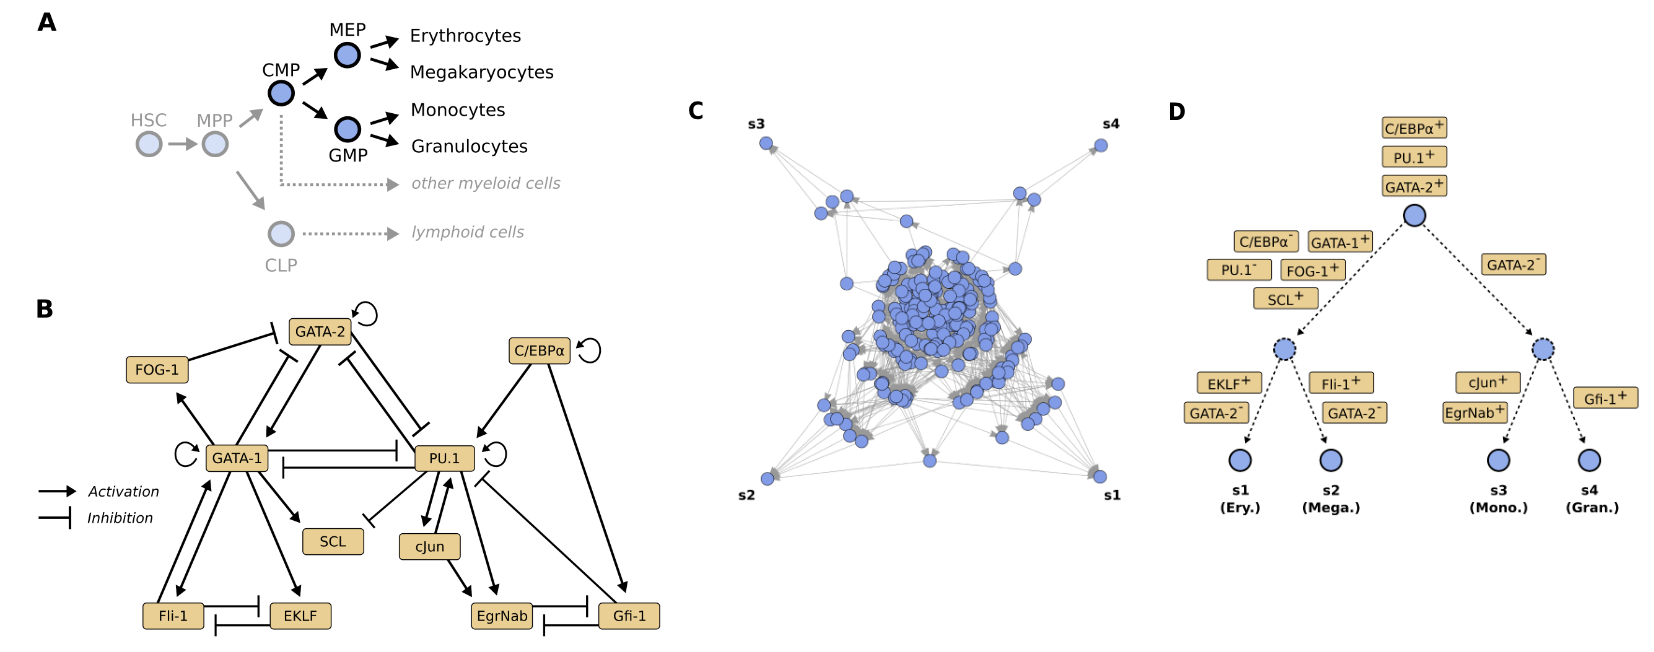
\includegraphics[width=\textwidth]{Figures/myeloid.png}
    \caption{\textbf{Myeloid cell differentiation.} From~\cite{Krumsiek2011}. The figure illustrates what differentiation process is exhibited by the model (A), the regulatory network of the model (B), a visualization of the state space of the model (C), and the deciding update factors driving a cell from common myeloid progenitor (CMP) to the specific phenotypes (D).}
    \label{fig:myeloid}
  	\end{minipage}
	}
\end{figure}

To demonstrate an example of how the control of \PBN{} can be applied to cell reprogramming, we consider a case study of myeloid cell differentiation. Myeloid cells are a type of blood cell that can differentiate into various cell types, including erythrocytes, megakaryocytes, monocytes, and granulocytes. Understanding the regulatory mechanisms underlying myeloid differentiation is crucial for developing therapies for diseases such as leukaemia and other blood disorders. We will be using model from~\cite{Krumsiek2011}. The model has 11 variables and its regulatory network along with the model semantics can be seen in the \autoref{fig:myeloid}. 

\sethlcolor{green!30}
\begin{table}[htbp!]
\small
\centering
\caption{\textbf{Attractor states of myeloid model}. All attractor sizes are 1 and represent four types of specialized blood cells. Values are binary and represent value assignments of model variables. The \hl{highlighted values} represent the differentiating factor for each cell type that is considered in the phenotype specification later.}
\label{tab:myeloid_attractors}
\begin{tabular}{p{1.3cm}w{c}{1.9cm}w{c}{2.3cm}w{c}{1.9cm}w{c}{1.9cm}}
\hline
 & \textbf{Erythrocyte} & \textbf{Megakaryocyte} & \textbf{Monocyte} & \textbf{Granulocyte} \\
\hline
CEBPa   & 0 & 0 & 0 & 1 \\
\cellcolor{green!30}EKLF    & \cellcolor{green!30}1 & 0 & 0 & 0 \\
EgrNab  & 0 & 0 & 1 & 0 \\
FOG1    & 1 & 1 & 0 & 0 \\
\cellcolor{green!30}Fli1    & 0 & \cellcolor{green!30}1 & 0 & 0 \\
GATA1   & 1 & 1 & 0 & 0 \\
GATA2   & 0 & 0 & 0 & 0 \\  
\cellcolor{green!30}Gfi1    & 0 & 0 & 0 & \cellcolor{green!30}1 \\
PU1     & 0 & 0 & 1 & 1 \\
SCL     & 1 & 1 & 0 & 0 \\
\cellcolor{green!30}cJun    & 0 & 0 & \cellcolor{green!30}1 & 0 \\
\hline
\label{tab:myeloid_attractors}
\end{tabular}
\end{table}

We use AEON.py~\cite{aeonpy} to do the analysis of the model and to compute the control. First, we do a standard attractor search to find the attractors of the model. The binary single-state attractors are shown in~\autoref{tab:myeloid_attractors}. Even though the tool does not tell us the semantics of the attractors, we can identify them by comparing the attractor states with the known phenotypes of the myeloid differentiation. The single differentiating factor for each cell type is highlighted in the table.

Since we have results from the attractor search, we can perform the source-target control for all the attractor pairs. The presumption is that eventually the cell converges to one of the possible attractors and that using source-target control we can find perturbations which can drive the cell from one attractor to another. The results of the control are shown in \autoref{tab:myeloid_st}. We can see that in some cases one-step perturbations are bigger than temporary or permanent perturbations. The worst case is reprogramming from megakaryocytes to granulocytes, where one-size perturbation needs to be of size 4 while temporary or permanent perturbation suffice with size 2. Also, even though temporary and permanent perturbation are of the same size, for some cases there are more options for temporary perturbations than for permanent ones.


\begin{table}[htb]
\centering
\footnotesize
\setlength{\tabcolsep}{4pt}
\checkoddpage
\edef\side{\ifoddpage l\else r\fi}
\makebox[\textwidth][\side]{% 
\begin{minipage}[t]{\fullwidth}
\caption{\textbf{Source-target control between attractors.} Perturbation values are written as $\var{x}\shorteq1$ (True) and $\var{x}\shorteq0$ (False). When a perturbation contains multiple assignments, they are grouped in braces $\{\cdot\}$.}
\resizebox{\textwidth}{!}{
\begin{tabular}{llp{4.6cm}p{4cm}p{4cm}}
\hline
\textbf{Source} & \textbf{Target} & \textbf{One-step} & \textbf{Temporary} & \textbf{Permanent} \\
\hline
Ery. & Mega.
& \{\var{EKLF}${\shorteq}0$,\var{Fli1}${\shorteq}1$\}
& \var{Fli1}${\shorteq}1$;\var{EKLF}${\shorteq}0$
& \var{Fli1}${\shorteq}1$;\var{EKLF}${\shorteq}0$ \\

Ery. & Mono.
& \var{PU1}${\shorteq}1$
& \var{PU1}${\shorteq}1$
& \var{PU1}${\shorteq}1$ \\

Ery. & Gran.
& \{\var{CEBPa}${\shorteq}1$,\var{GATA1}${\shorteq}0$,\var{Gfi1}${\shorteq}1$\}
& \{\var{CEBPa}${\shorteq}1$,\var{cJun}${\shorteq}0$\};\
& \{\var{CEBPa}${\shorteq}1$,\var{cJun}${\shorteq}0$,\var{Gfi1}${\shorteq}1$\}\\
& & & \{\var{CEBPa}${\shorteq}1$,\var{EgrNab}${\shorteq}0$\}; & \{\var{CEBPa}${\shorteq}1$,\var{EgrNab}${\shorteq}0$\}; \\
& & & \{\var{CEBPa}${\shorteq}1$,\var{Gfi1}${\shorteq}1$\} & \{\var{CEBPa}${\shorteq}1$,\var{Gfi1}${\shorteq}1$\}\\

Mega. & Ery.
& \{\var{EKLF}${\shorteq}1$,\var{Fli1}${\shorteq}0$\}
& \var{Fli1}${\shorteq}0$;\ \var{EKLF}${\shorteq}1$
& \var{Fli1}${\shorteq}0$;\ \var{EKLF}${\shorteq}1$ \\

Mega. & Mono.
& \var{PU1}${\shorteq}1$
& \var{PU1}${\shorteq}1$
& \var{PU1}${\shorteq}1$ \\

Mega. & Gran.
& \{\var{CEBPa}${\shorteq}1$,\var{Gfi1}${\shorteq}1$,\var{PU1}${\shorteq}1$,\var{SCL}${\shorteq}0$\}
& \{\var{CEBPa}${\shorteq}1$,\var{cJun}${\shorteq}0$\};\ 
& \{\var{CEBPa}${\shorteq}1$,\ \var{cJun}${\shorteq}0$\};\ \\

&  & \{\var{CEBPa}${\shorteq}1$,\var{Gfi1}${\shorteq}1$,\var{PU1}${\shorteq}1$,\var{GATA1}${\shorteq}0$\} & \{\var{CEBPa}${\shorteq}1$,\var{EgrNab}${\shorteq}0$\}; & \{\var{CEBPa}${\shorteq}1$,\var{EgrNab}${\shorteq}0$\};  \\
&  & \{\var{CEBPa}${\shorteq}1$,\var{Gfi1}${\shorteq}1$,\var{Fli1}${\shorteq}0$,\var{GATA1}${\shorteq}0$\} & \{\var{CEBPa}${\shorteq}1$,\var{Gfi1}${\shorteq}1$\} & \{\var{CEBPa}${\shorteq}1$,\var{Gfi1}${\shorteq}1$\} \\

Mono. & Ery.
& \{\var{EKLF}${\shorteq}1$,\var{GATA1}${\shorteq}1$,\var{PU1}${\shorteq}0$\}
& \{\var{Fli1}${\shorteq}0$,\ \var{GATA2}${\shorteq}1$,\ \var{PU1}${\shorteq}0\};\ \dots$
& \{\var{Fli1}${\shorteq}0$,\ \var{GATA2}${\shorteq}1$,\ \var{PU1}${\shorteq}0\};\ \dots$ \\
& & & $\dots$ \textit{5 more options} & \{\var{EKLF}${\shorteq}1$,\ \var{GATA2}${\shorteq}1$,\ \var{PU1}${\shorteq}0$\};\ \\

Mono. & Mega.
& \{\var{Fli1}${\shorteq}1$,\var{GATA1}${\shorteq}1$,\var{PU1}${\shorteq}0$\}
& \{\var{PU1}${\shorteq}0$,\ \var{Fli1}${\shorteq}1$\}
& \{\var{Fli1}${\shorteq}1$,\ \var{PU1}${\shorteq}0$\} \\

Mono. & Gran.
& \{\var{CEBPa}${\shorteq}1$,\var{EgrNab}${\shorteq}0$,\var{Gfi1}${\shorteq}1$\}
& \{\var{CEBPa}${\shorteq}1$,\ \var{cJun}${\shorteq}0$\};
& \{\var{CEBPa}${\shorteq}1$,\ \var{cJun}${\shorteq}0$\}; \\
& & & $\dots$ \textit{3 more options} & $\dots$ \textit{2 more options} \\

Gran. & Ery.
& \{\var{CEBPa}${\shorteq}0$,\var{EKLF}${\shorteq}1$,\var{GATA1}${\shorteq}1$,\var{PU1}${\shorteq}0$\} 
& \{\var{Fli1}${\shorteq}0$,\var{GATA2}${\shorteq}1$,\var{PU1}${\shorteq}0$\};\ $\dots$
& \{\var{Fli1}${\shorteq}0$,\var{GATA2}${\shorteq}1$,\var{PU1}${\shorteq}0$\};\  \\
& & & $\dots$ \textit{5 more options} & \{\var{EKLF}${\shorteq}1$,\var{GATA2}${\shorteq}1$,\var{PU1}${\shorteq}0$\} \\

Gran. & Mega.
& \{\var{CEBPa}${\shorteq}0$,\var{GATA1}${\shorteq}1$,\var{Fli1}${\shorteq}1$,\var{PU1}${\shorteq}0$\} 
& \{\var{PU1}${\shorteq}0$,\ \var{Fli1}${\shorteq}1$\} 
& \{\var{Fli1}${\shorteq}1$,\ \var{PU1}${\shorteq}0$\} \\

Gran. & Mono.
& \var{CEBPa}${\shorteq}0$ 
& \var{CEBPa}${\shorteq}0$ 
& \var{CEBPa}${\shorteq}0$ \\
\hline
\end{tabular}}
\label{tab:myeloid_st}
\end{minipage}}
\end{table}


\begin{figure}
  \centering
  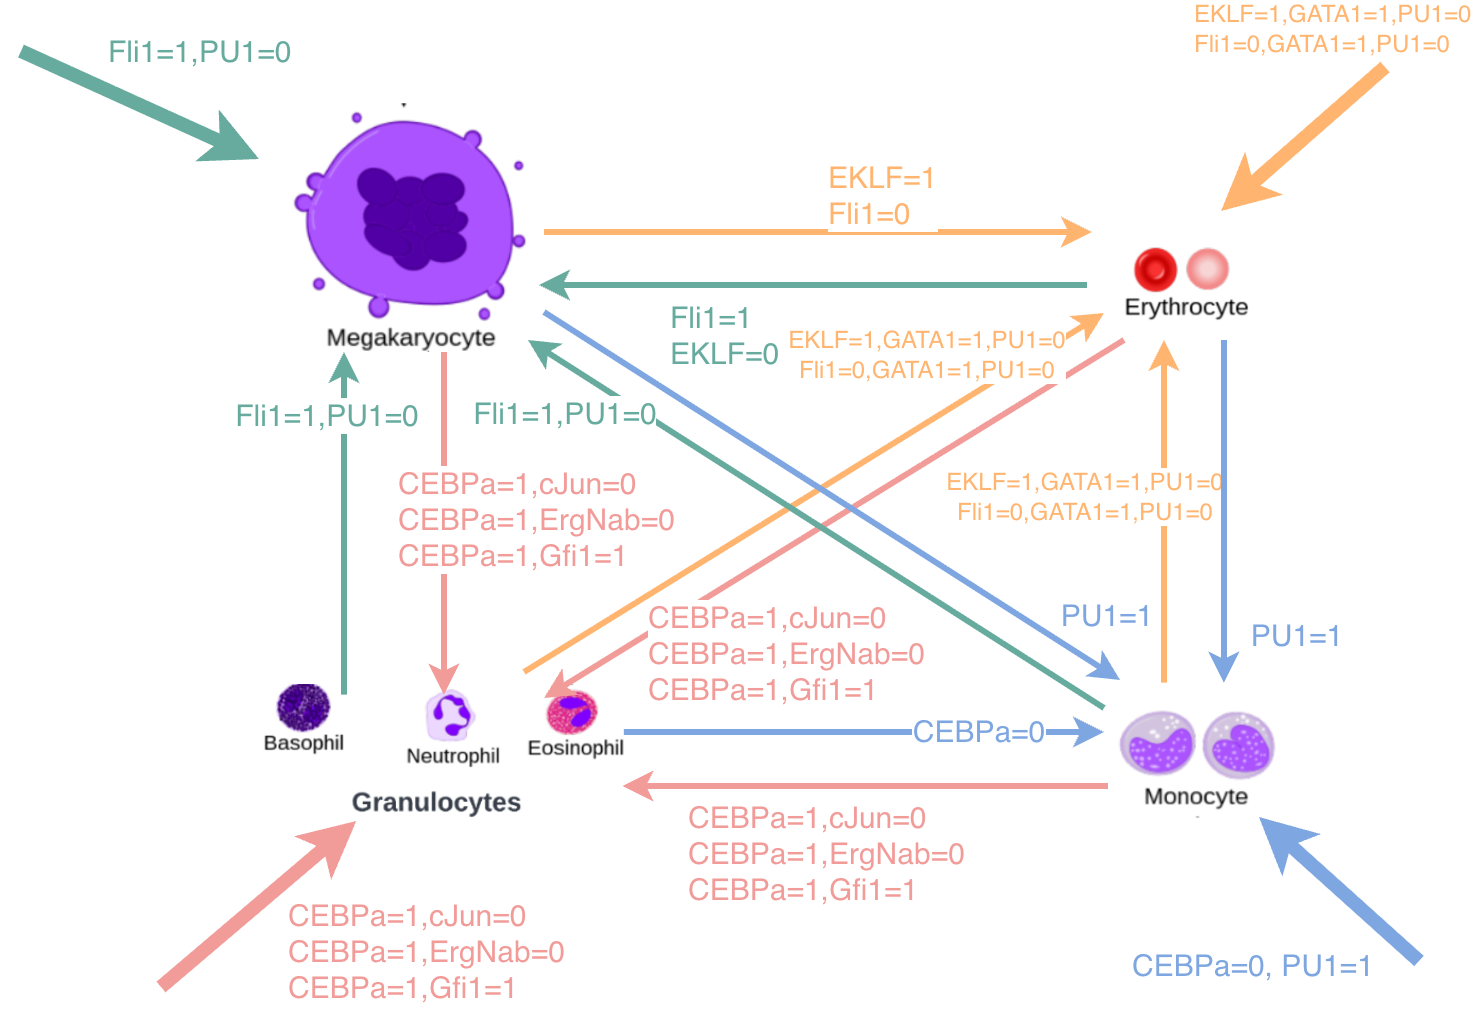
\includegraphics[width=0.9\textwidth]{Figures/myeloid_phenotype.png}
  \caption{\textbf{Control results for myeloid model.} The figure shows the results of control for each cell type in the myeloid model. The arrows going from one cell type to another represent results of permanent source-target control while the arrows going into a cell type (without any source) show results of phenotype control. Each row of the arrow label represents one perturbation. The color of each arrow depends on the control's target -- green for megakaryocytes, blue for monocytes, orange for erythrocytes and red for granulocytes.}
  \label{fig:myeloid_full_control}
\end{figure}

Next, we can also run phenotype control to find the perturbations that stabilize the network regardless of the source attractor. The results of the phenotype control are shown in \autoref{fig:myeloid_full_control}. We can see, that in some cases, like in case of megakaryocytes, the minimal perturbation size is the same for source-target and phenotype control, while with control to other cell types we can fine-tune the perturbation to the known source and use a subset of the complete phenotype perturbation. Nonetheless, the phenotype control is always a superset of the source-target control, which is consistent with the fact that the phenotype control is a more general problem.

Finally, we can briefly compare our results with the source paper of the model that is depicted in \autoref{fig:myeloid}. We can see, that our framework yielded results consistent with the original study, since no perturbation negates the perturbation evolution depicted in branches (the root is only initial state and it can be negated). Sometimes, the negation of factors that are driving to one cell type work as a driver to another cell type, which is consistent with the known biology of the system. For example, the perturbations to erythrocytes can be enabled either by over-expression of EKLF (as depicted in the original study) or by the knock-out of Fli1 which over-expression is driving to megakaryocytes.

\begin{table}[htbp!]
\small
\caption{\textbf{Functions of partially specified myeloid model.} The functions of the original model are shown in the second column, while the functions of the partially specified model are shown in the third column. The symbol `---' means, that the function is not changed. The new functions are defined as functions of the original variables and thus they are consistent with the original model.}
\centering
\begin{tabular}{lll}
\hline
\textbf{Variable} & \textbf{Function} & \textbf{New function}\\
\hline
\var{GATA2} & $\var{GATA2} \land \neg(\var{GATA1} \land \var{FOG1}) \land \neg{\var{PU1}}$ & $f(\var{GATA2}, \var{GATA1}, \var{FOG1}, \var{PU1})$ \\
\var{GATA1} & $(\var{GATA1} \lor \var{GATA2} \lor \var{Fli1}) \land \neg{\var{PU1}}$ &  --- \\
\var{FOG1} & $\var{GATA1}$ & --- \\
\var{EKLF} & $\var{GATA1} \land \neg\var{Fli1}$ & --- \\
\var{Fli1} & $\var{GATA1} \land \neg\var{EKLF}$ & --- \\
\var{SCL} & $\var{GATA1} \land \neg\var{PU1}$ & --- \\
\var{CEBPa} & $\var{CEBPa} \land \neg(\var{GATA1} \land \var{FOG1} \land \var{SCL})$ & $g(\var{CEBPa}, \var{GATA1}, \var{FOG1}, \var{SCL})$ \\
\var{PU1} & ($\var{CEBPa} \lor \var{PU1}) \land \neg(\var{GATA1} \lor \var{GATA2})$ & $h(\var{CEBPa}, \var{PU1}, \var{GATA1}, \var{GATA2})$ \\
\var{cJun} & $\var{PU1} \land \neg\var{Gfi1}$ & --- \\
\var{EgrNab} & $(\var{PU1} \land \neg\var{cJun}) \land \neg\var{Gfi1}$ & --- \\
\var{Gfi1} & $\var{CEBPa} \land \neg\var{EgrNab}$ & --- \\
\hline
\label{tab:myeloid_funs}
\end{tabular}
\end{table}

In order to fully demonstrate the capability of the developed methods, we decided to simulate partial specification of the model by arbitrarily introducing some unknown functions in the model. The model adjustments can be seen in \autoref{tab:myeloid_funs}.


\begin{figure}[htbp!]
  \centering
  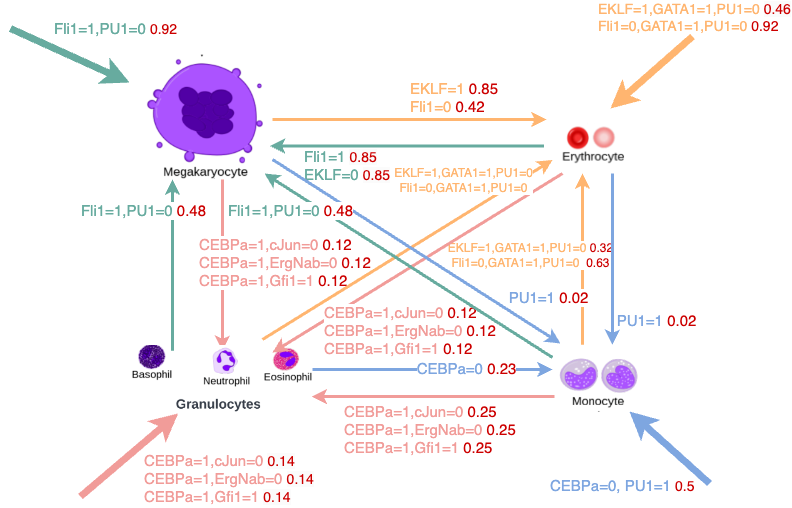
\includegraphics[width=\textwidth]{Figures/myeloid_perturbations_robustness.png}
  \caption{\textbf{Control results for partially specified myeloid model.} The figure shows the results from \autoref{fig:myeloid_full_control} in the partially specified model. The considered perturbations are the equal to the ones in the fully specified model, but they are also labelled with the robustness in the partially specified model.}
  \label{fig:myeloid_full_control_adjusted}
\end{figure}

However, attractor analysis of the partially specified model revealed that some attractors satisfy multiple phenotype specifications when phenotypes are defined by the expression of a single marker. For example, there was an attractor that had \var{EKLF}$\shorteq1$ and $\var{Gfi1}\shorteq1$, therefore it was shared between erythrocytes and granulocytes. To resolve this issue, we adjust the phenotype specification to require only one marker to be set to true, while other markers were required to be false. For example, the phenotype specification for erythrocytes was changed from $\var{EKLF}\shorteq1$ to $\var{EKLF}\shorteq1 \land \var{Fli1}\shorteq0 \land \var{Gfi1}\shorteq0 \land \var{cJun}\shorteq0$. This adjustment ensured that the phenotypes are disjoint, and thus we can perform the control analysis without any issues. The results of the control in the partially specified model are shown in \autoref{fig:myeloid_full_control_adjusted}. 

What is interesting, is that phenotype control in some cases, despite being global and therefore solving a harder problem in a sense has more robust perturbation than source-target control (for example, for megakaryocytes or monocytes). This is because the source-target control is more restrictive and requires stabilization in one specific state, while the phenotype control requires stabilization allows for stabilization in any state of the phenotype, which is more flexible and robust toward model uncertainty. This well illustrates the advantage of the phenotype control over the source-target control in the context of model uncertainty. 

In this section we have seen, that introducing uncertainty into the model can lead to unexpected behaviors of the model, such as shared attractors between phenotypes. This can be seen as an example of how the model uncertainty can lead to a loss of model precision. In the next section, we will show how the control can be used to guide the model refinement and thus to lower the model uncertainty and increase the model precision.


\section{Control workflow for therapy and model refinement}
\label{sec:control_workflow}

\begin{figure}[htbp!]
\checkoddpage
\edef\side{\ifoddpage l\else r\fi}
\makebox[\textwidth][\side]{% 
	\begin{minipage}{\fullwidth}
    \centering
    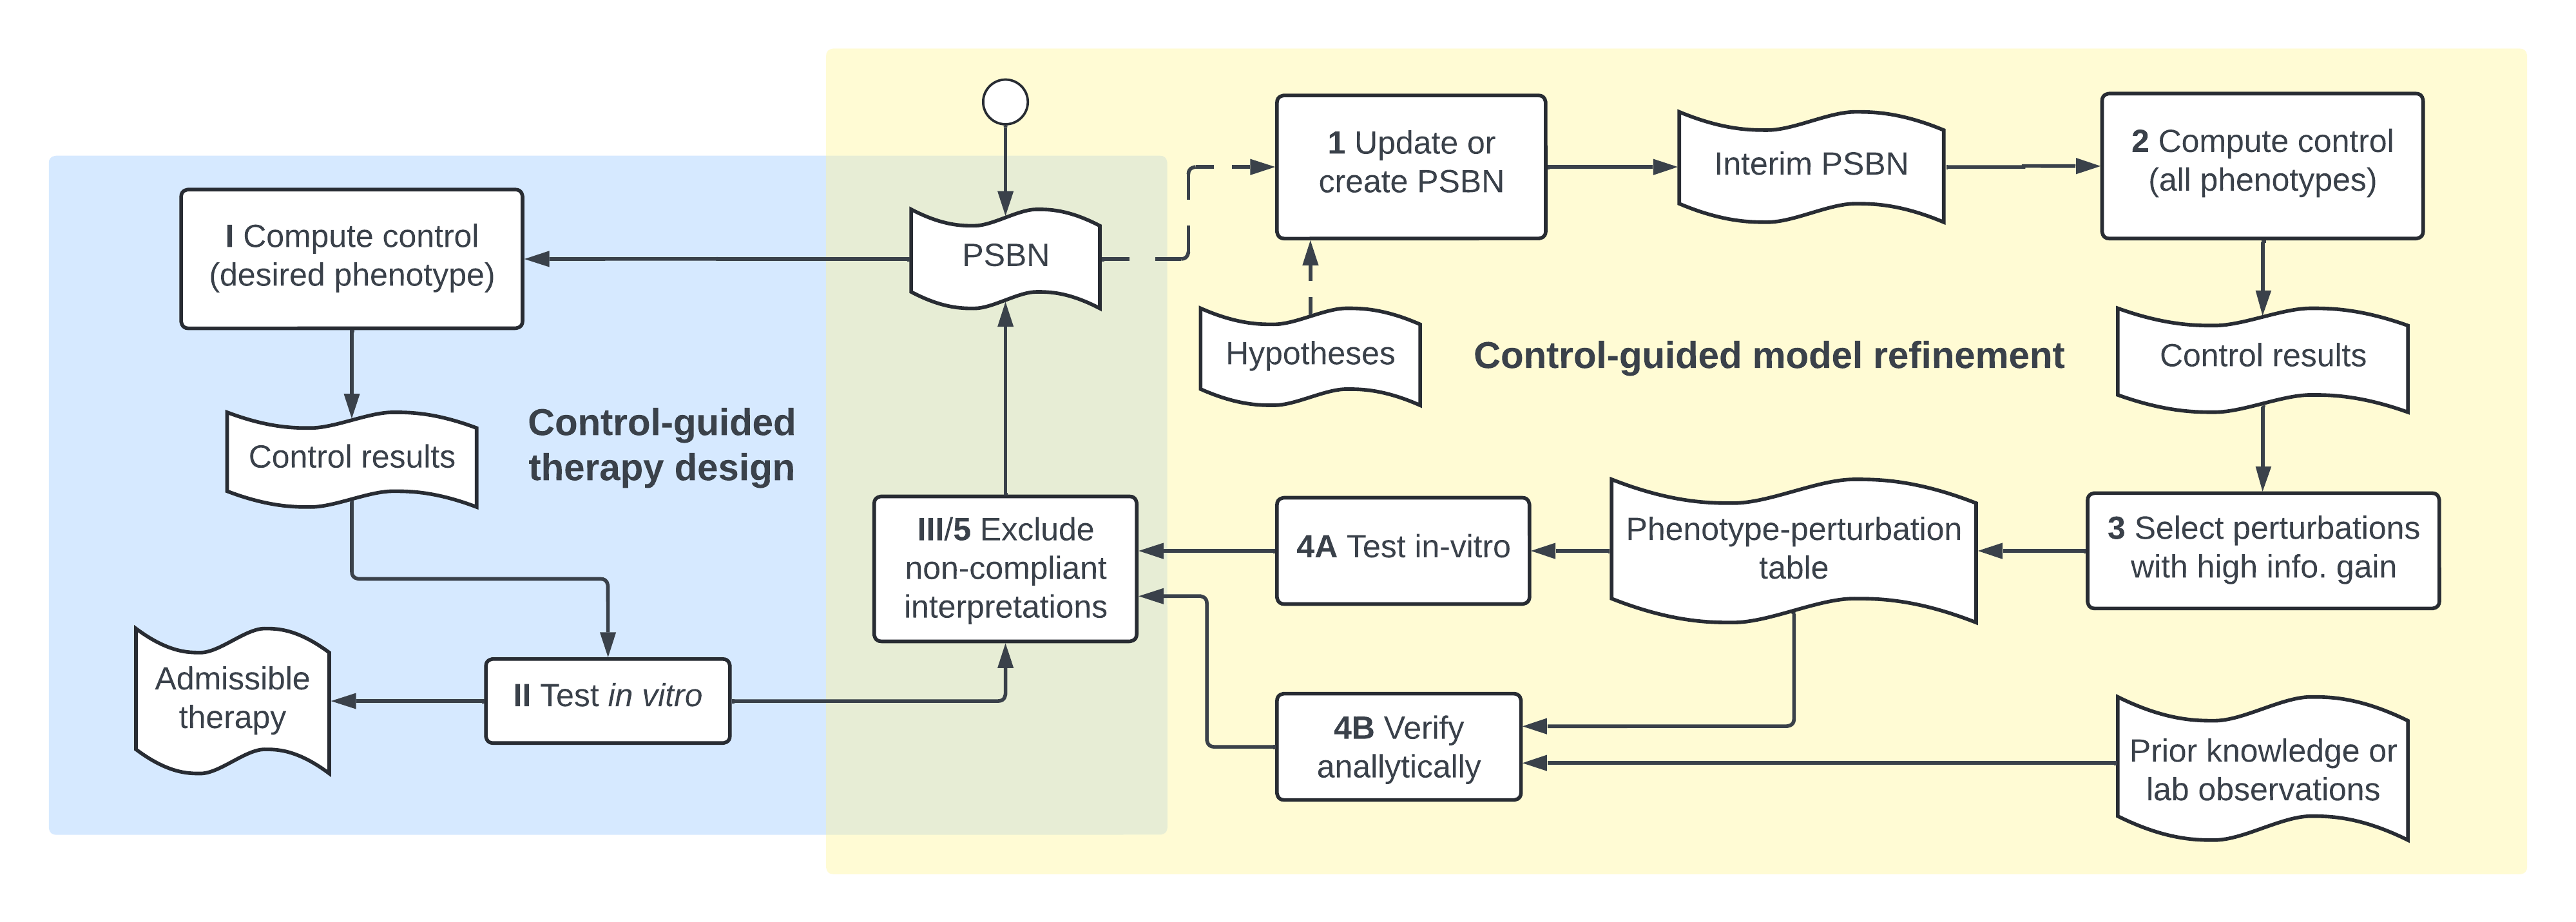
\includegraphics[width=\textwidth]{Figures/control_workflow3.png}
    \caption{\textbf{Workflows of control framework.} The diagram in the picture depicts two workflows of how the phenotype control can be used to achieve two different goals -- to find a therapy or to refine a PSBN model. The workflows can be combined or achieve each other's goals as a side effect (e.g., we might refine model after refuting that the obtained therapy works). The rectangle boxes represent the steps of the workflow, while the tape shaped boxes represent the artifacts obtained from the conducted steps.}
    \label{fig:control_workflow}
  	\end{minipage}
	}
\end{figure}

In this section, we will zoom in on the practical workflow of how the control of partially specified Boolean networks can be used to design a therapy or to refine the model. The workflow is depicted in \autoref{fig:control_workflow}. We will explain the two main branches of the workflow -- control-driven therapy design and control-guided model refinement. We will also show how these two branches can be combined and how they can benefit each other.

\subsection{Control-driven therapy design}

In the previous sections, we have demonstrated the application of \PBN{}  control in context of cell reprogramming. In general, we can refer to this process as \emph{therapy design} in case the goal is to find a suitable treatment which achieves a desired (healthy) system behavior~\cite{Bloomingdale2018, Kim2017, Mendez2017,Saadatpour2011, Zhu2016}. 

Also, as we have seen that such an objective can be directly translated to the phenotype control problem where the system behavior is described via PSBN and the target behavior via a phenotype. The output of the control problem is a set of perturbations which can be implemented back to the real-world, for example as gene knockouts and over-expressions. 


In an ideal case, the artifact obtained from this workflow is a therapy design that can be proven to work in in-vitro (or in-vivo) experiments. Usually, the preferred perturbations are the ones which are easiest to implement in practice (i.e., with the smallest perturbations or the ones which are the most biologically feasible)~\cite{Su2019CMSB}. The second criterion to consider is an expected chance of the therapy to work. This aspect is estimated by the model via a robustness metric of the perturbation~\cite{brim2022}. 

Nonetheless, since the model is imprecise to some extent, the designed therapy might not work in practice. In such case the observations from the experiment can be used to refine \PBN{} model. Usually, we can simply refute the interpretations which do not comply with obtained observation. For example, if we expected a perturbation \var{FGFR3}=1 to stabilize the network in a phenotype \var{ERK}=1 for 60\% of interpretations, but the real-world experiment do not stabilize this phenotype under \var{FGFR3} over-expression, we can conclude, that these 60\% of interpretations are not representing the studied system correctly, and thus we can discard them from the considered set of interpretations. This would complete the workflow cycle depicted on the left side of the diagram in \autoref{fig:control_workflow} and we can attempt to recompute the therapy design with the remaining interpretations.

\subsection{Control-guided model refinement}

In more complex cases, it is also possible, that the treatment is not replicated in vitro even for a perturbation with 100\% robustness. As a result, we might need to rework the model significantly, e.g., by introducing new model parts (regulations and variables) or by changing the existing components. Typically, these model adjustments significantly expand unknown parts of the model, since they are based on hypotheses and uncertainty. Then, a typical next step is verification of the hypotheses we posed as well as efforts to lower the introduced uncertainty. 

As shown on the right side of the diagram in \autoref{fig:control_workflow}, we use phenotype control to guide an experimental design of knockout or over-expression experiments for the model refinement~\cite{UdDean2016}. Let us zoom in to the details of this process.

\paragraph{Initial \PBN{} model}
We start with an initial \PBN{} model (Step 1; Fig. \autoref{fig:control_workflow}) and its phenotypes. Such \PBN{} can be constructed directly from prior knowledge and known assumptions about biological behavior, or it can be an extension of some existing model relying on new information (e.g., newly discovered regulations or pathways).

\paragraph{Screening admissible perturbations}
We analyze the feasible perturbations w.r.t. known phenotypes of the \PBN{} (Step 2; \autoref{fig:control_workflow}). In therapy design, we would seek perturbations of high robustness achieving our phenotype of interest. For refinement, perfect robustness (i.e., $\rho(Q) = 1.0$) is \emph{not} desirable as it means the perturbed interpretations are indistinguishable through phenotype observations. Similarly, if two perturbations achieve equivalent phenotypes across all interpretations, only one needs to be considered further.

\paragraph{Selection of perturbations using information-gain}

While the initial screening can significantly reduce the space of admissible perturbations, it likely still remains too large to explore \emph{in vitro}. We therefore prioritize perturbations using a \emph{normalized mutual information score} (NMIS; \cite{Kent83}), quantifying how well is the outcome of a perturbation explained by a specific unknown \emph{feature} of the \PBN{} (Step 3;  \autoref{fig:control_workflow}). We use the following formulas to compute the NMIS:

$$
IS(X; Y) = \sum_{x, y} P(x, y) \log \frac{P(x, y)}{P(x) P(y)}
$$
$$
H(X) = -\sum_{x} P(x) \log P(x)
$$
$$ 
NMIS(X; Y) = \frac{2 IS(X; Y)}{H(X) H(Y)} 
$$

To compute NMIS, we observe that interpretations $\allInterpretations$ can be partitioned into equivalence classes $\interpretationSet_1, \ldots, \interpretationSet_k$ based on their outcomes, with each class consisting of interpretations that are indistinguishable by any admissible perturbation. Each class is assigned a set of \emph{behavior labels} and \emph{feature values}. 

Here, behavior labels correspond to the phenotypes observed when subject to individual perturbations (collectively, we call these the \emph{behavior pattern} of $\interpretationSet_i$). Similarly, \emph{feature values} are based on selected properties of the underlying class of networks~$\interpretationSet_i$. These features are derived from the unknown elements of the \PBN{}, such as the uninterpreted update functions or properties of regulations (essentiality, monotonicity, canalization, etc.).

We use NMIS to express the mutual information between the behavior labels achieved by a perturbation $Q$ and the values given by a particular network feature, quantifying how well the network feature predicts the outcome of perturbation $Q$.

High NMIS for a feature-perturbation pair indicates that observing the perturbed phenotypes should (with high likelihood) either confirm or refute that network feature. The perturbation with the highest NMIS (for some network feature) is selected for \emph{in vitro} testing (Step 4A; Fig.~\ref{fig:control_workflow}). Alternatively, prior knowledge can be introduced to assert the expected phenotypes of the model under perturbation (Step 4B; Fig.~\ref{fig:control_workflow}).

Finally, model instances that do not conform to the expected behavior are excluded (Step 5; Fig.~\ref{fig:control_workflow}), allowing us to restart the workflow with an updated \PBN{}.


% As opposed to the therapy design, in this case, we typically focus on perturbations which are the most informative, i.e., the ones which will help us to distinguish between the interpretations the most. More specifically, a perturbation which works for exactly same interpretations is not very informative, since we expect, that it works for all interpretations and thus would not help us lower the model uncertainty (number of interpretations). 

\paragraph{Example of perturbation selection}

For example, let us suppose, that we consider some \PBN{} $\pbnMath$ \emph{similar} to the one from example in \autoref{fig:psbn} (i.e., a \PBN{} with multiple variables and functional symbols). The \PBN{} has 2820 interpretations. and that we compute stabilization in prolifertion (P) phenotype. The result of the control could be perturbations $\perturbation_A, \perturbation_B, \perturbation_C$, while the union of the interpretations for which they work is exactly $\allInterpretations(\pbnMath)$. The cardinality and intersection of the interpretations they cover are shown in \autoref{subfig:set_example}. 

\begin{figure}[ht!]
  \checkoddpage
  \edef\side{\ifoddpage l\else r\fi}
  \makebox[\textwidth][\side]{% 
	\begin{minipage}[t]{\fullwidth}
  \centering
  \subfloat[Interpretation sets controlled by perturb. $\perturbation_A, \perturbation_B, \perturbation_C$.]{
    \begin{minipage}[t]{0.35\textwidth}
      \label{subfig:set_example}
      \vspace{-50pt}% <-- forces top alignment
      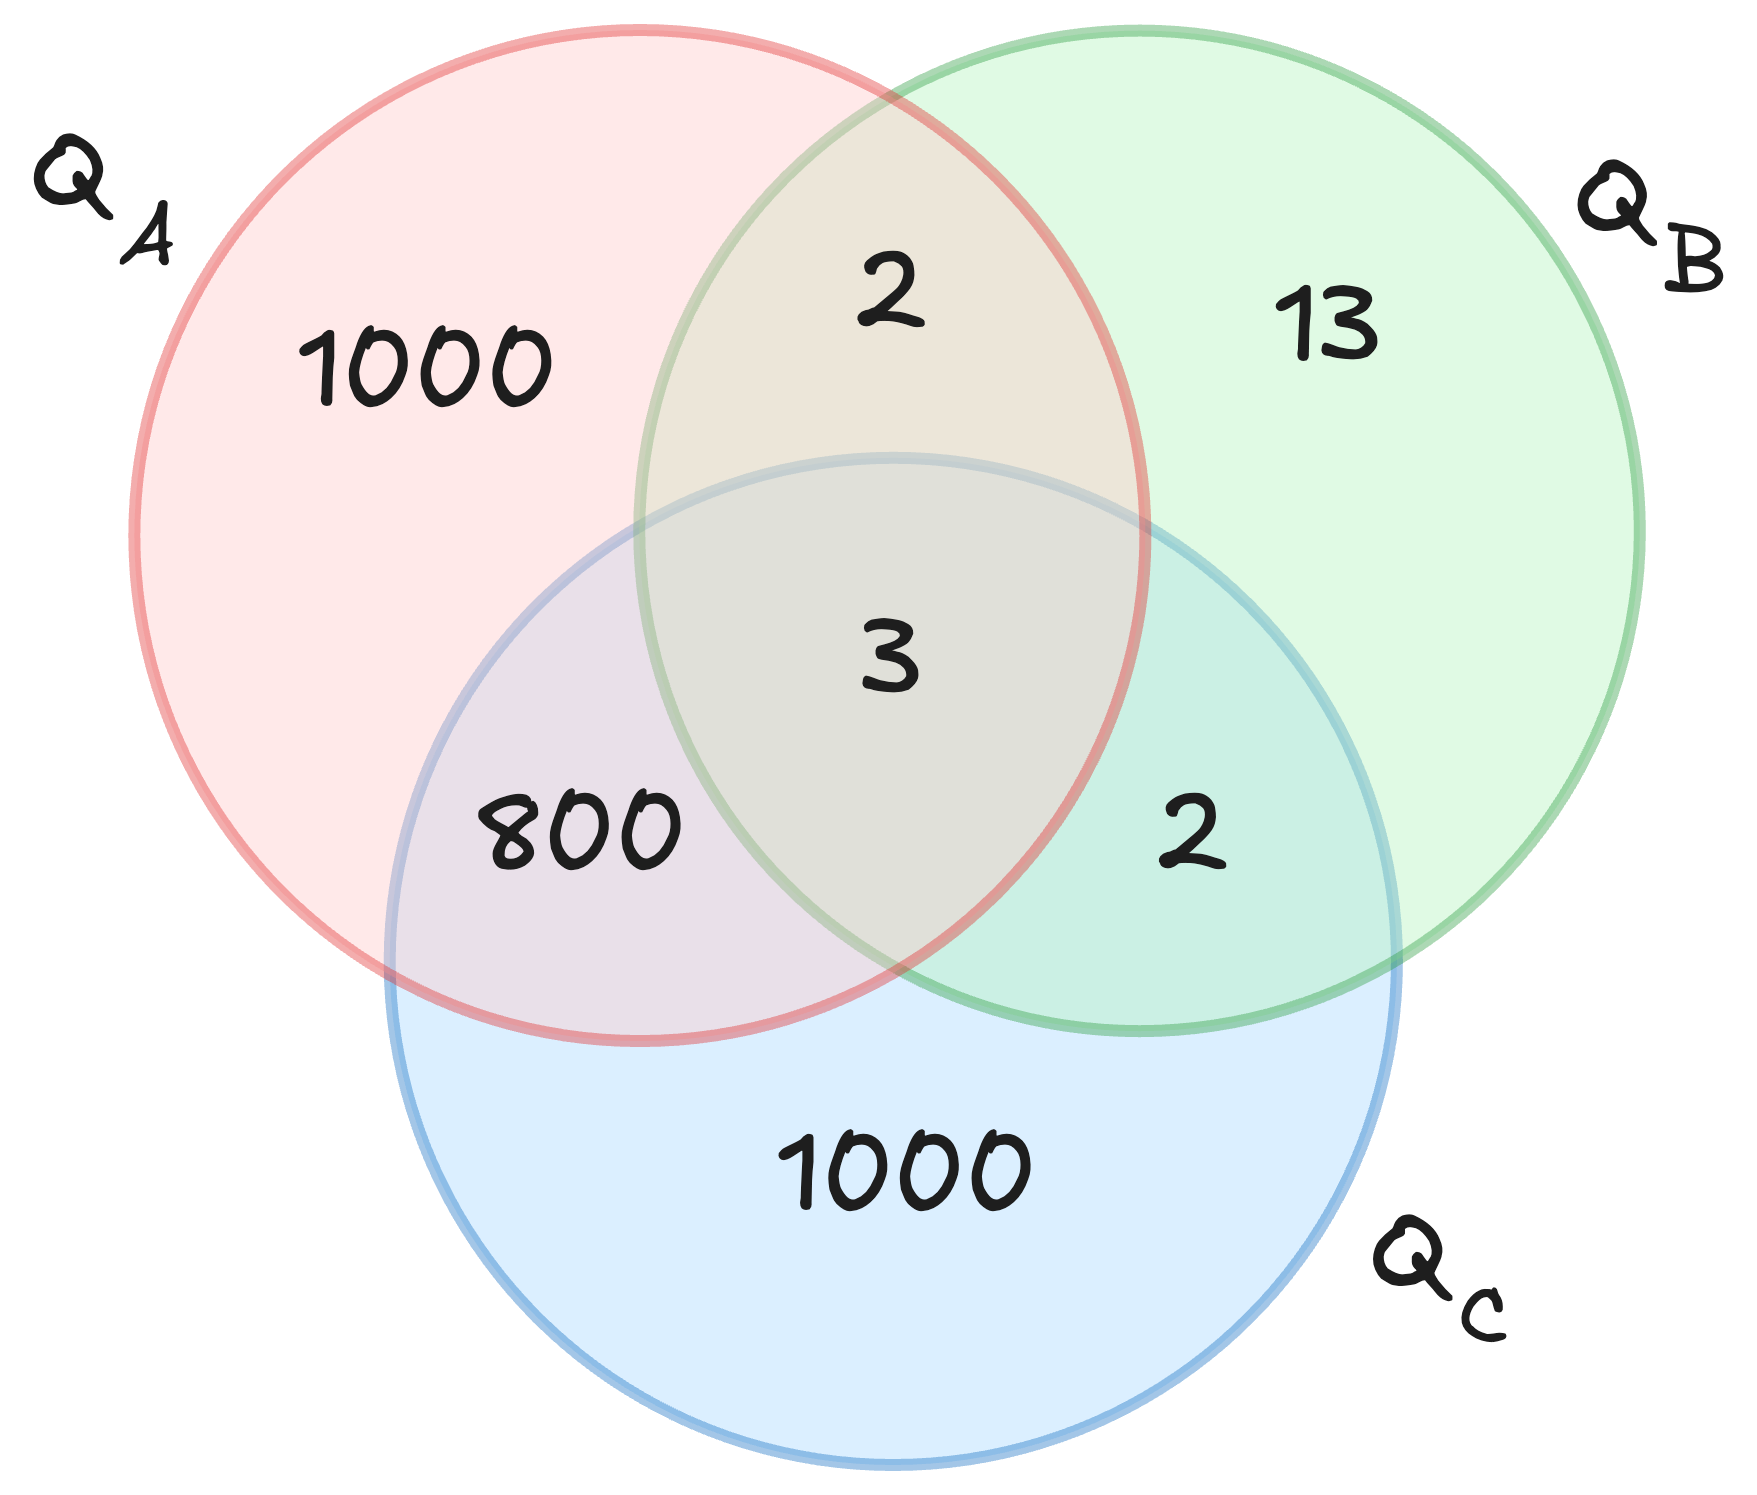
\includegraphics[width=\textwidth]{Figures/perturbations_venn_example.png}
    \end{minipage}
  }~~~~~~~~~~~~~~
  \subfloat[Phenotype-perturb. table for selection of $\perturbation_A$ and $\perturbation_B$.]{
    \begin{minipage}[b]{0.2\textwidth}
      \begin{tabular}{ccl}
      $Q_A$ & $Q_B$ & $\mid \interpretationSet \mid$ \\
      P     & P     & 5               \\
      P     & A  & 1800            \\
      A     & P    & 15              \\
      GA     & A    & 1000           
      \end{tabular}
    \end{minipage}
    \label{subfig:select_a_b}
  }~~~~~~~~~~~~~~
  \subfloat[Phenotype-perturb. table for selection of $\perturbation_A$ and $\perturbation_C$.]{
  \begin{minipage}[b]{0.2\textwidth}
    \begin{tabular}{ccl}
      $\perturbation_A$ & $\perturbation_C$ & $\mid \interpretationSet \mid$ \\
      P    & P & 803             \\
      P    & A  & 1002            \\
      A    & P   & 1002            \\
      A    & A  & 13             
      \end{tabular}
    \end{minipage}
    \label{subfig:select_a_c}
  }
  \vspace*{2mm}
  \caption{
    \textbf{An example of interpretations partitioning of working perturbations.} \autoref{sub@subfig:set_example} shows sets of interpretations and their intersections for some three distinct perturbations $\perturbation_A, \perturbation_B, \perturbation_C$. Then, the \autoref{sub@subfig:select_a_b} and \autoref{sub@subfig:select_a_c} show phenotype-perturbation matrices if perturbations $\perturbation_A$ and $\perturbation_B$ are selected or $\perturbation_A$ and $\perturbation_C$ respectively. Each row represents a set of interpretations. The values in the table cells contain a phenotype in which model stabilizes under the given perturbation one of proliferation (P), apoptosis (A) or growth arrest (GA). The last column contains cardinality of the relevant interpretation set.}
  \label{fig:perturbations_example}
  \end{minipage}
  }
\end{figure}

We can notice, that despite the perturbations $\perturbation_A$ and $\perturbation_C$ are working for exactly the same amount of interpretations, they might control very different sets of particular interpretations. If there would be multiple perturbations which work for exactly same interpretations as the perturbation $\perturbation_A$, it is not expected to be informative to use them all in the real-world experiments. Finally, we can see, that the perturbation $\perturbation_B$ is also covering distinct sets of perturbations, although their size is much smaller. 

If we were in the situation, when we would need to select only two perturbations for the real-world experiments (e.g, due to the high experiment price) we can consider the reduced interpretation sets in \emph{perturbation-phenotype tables} depicted in \autoref{subfig:select_a_b} and \autoref{subfig:select_a_c}. The rows of these tables represent non-overlapping interpretation \emph{classes} with distinct \emph{behavior patterns}, while column values show differing phenotype outcomes of these interpretations under the selected perturbations.

When deciding which two perturbations out of three should be kept, we would be probably inclined to select $\perturbation_A$ and $\perturbation_C$ since in the worst (and most probable) case we would reduce the model uncertainty to a third of the original interpretation cardinality. On the other hand, if we would select $\perturbation_A$ and $\perturbation_B$, there would be a chance, that we would reduce the model uncertainty to a very small fraction of the original one, but the expected chances of this are very low. Nonetheless, the in ideal scenario we would be able to try all three perturbations in the real-world experiments, or we would prefer the perturbations which are easier to implement. 

Notice, that in phenotype-perturbation matrix we may not just represent whether the perturbation works or not, but also which phenotype in particular it exhibits. This is particularly useful for the model refinement, since we can then distinguish behavior classes depending on the exhibited phenotype.

Therefore, this table can be then directly used for design of knock-out and over-expression experiments in the real world. Since rows of a table always contain a distinct combination of phenotypes, we expect to be able to match the results from the phenotypes observed in the real-world to one particular row of the phenotype-perturbation table and thus significantly reduce the model uncertainty.

Performing the designed experiments in vitro is an ideal approach to refine the model. However, the experiments are usually costly and might not always be possible to implement. In such cases, we can still observe which model mechanics allow or prevent a perturbation working for some interpretations. For this, purpose, we can infer \emph{features} of an interpretation sets split obtained in the previous step. 

\begin{table}[ht!] 
  \centering
  \begin{tabular}{l|cc|cc}
                  & \multicolumn{2}{c|}{\textbf{Perturbations}} & \multicolumn{2}{c}{\textbf{Features}}                                     \\
  $\mid \interpretationSet \mid$ & $\perturbation_A$ & $\perturbation_C$ & $\exists \interpretation \in \interpretationSet.$ \var{ERK} $\rightarrow$ \var{FRS2} & $\forall \interpretation \in \interpretationSet . \var{FGFR3} = 0$ \\
  \hline
   803  & P & P & 1 & 0 \\
   1002 & P & A & 0 & 1 \\
   1002 & A & P & 0 & 0 \\
   13   & A & A & 0 & 1                         
  \end{tabular}
  \caption{\textbf{Example of phenotype-perturbation tables with extracted features.} The table shows the binarized  phenotype-perturbation table for the perturbations $\perturbation_A$ and $\perturbation_C$ from \autoref{fig:perturbations_example}. The table is extended with features extracted from the interpretation sets.}
  \label{tab:perturbation_matrix}
  \end{table}

For example, consider \autoref{tab:perturbation_matrix}, where we have selected two perturbations from the previous example in \autoref{fig:perturbations_example}. In the table, we assume that we have selected perturbations $\perturbation_A$ and $\perturbation_C$. We might be interested in finding out \emph{why} a particular perturbation works for some interpretations and not for the others. For this purpose, we infer the features of the interpretation sets. The vector of phenotypes for perturbations can thus be considered as a \emph{label}, and we can observe their \emph{mutual information gain} metric to measure impact of a feature on the~\cite{Kent83}. Note, that since question we are interested in is whether a perturbation works or not, thus it is more advantageous to consider binary labels (yes/no) for the labels. 
Given a set of interpretations $\interpretationSet$, the features we consider are following:
\begin{itemize}
  \item A regulation is essential in all interpretations $\forall \interpretation \in \interpretationSet.$ \var{GRB2} $\rightarrow$ \var{FGFR3} is observable in \pbnMath(\interpretation).
  \item A regulation is essential in any interpretation $\exists \interpretation \in \interpretationSet.$ \var{GRB2} $\rightarrow$ \var{FGFR3} is observable in \pbnMath(\interpretation).
  \item A presence of a particular function instance in 
  all of the given interpretations ($\forall \interpretation \in \interpretationSet .$\var{FGFR3} $=$ \var{FGFR3\_stimulus} $\land$ $\neg$\var{GRB2}  in \pbnMath(\interpretation)). This way we learn, that a particular function is necessary for the phenotype control to work.
  \item A presence of a particular function instance in any of the given interpretations ($\exists \interpretation \in \interpretationSet.$ \var{FGFR3} $=$ \var{FGFR3\_stimulus} $\land$ $\neg$\var{GRB2} in \pbnMath(\interpretation)). This way we might find, that a particular function is preventing a perturbation from working.
\end{itemize}

Note, that the features can be combined in various ways as well as there might be other features to consider (e.g. monotonity of regulations, or particular values of the function symbols, etc.). A rule of the thumb is to refine as many potentially relevant features as possible. In our example, we can notice, that perturbation $\perturbation_C$ avoids proliferation exactly if an interpretation has update function $\var{FGFR3}$=0. This could be a surprising observation for the modeler since maybe they did not expect $\var{FGFR3}$ function to be so trivial, nor $\perturbation_C$ to have such effect on proliferation. If such is the case, approximately a third of the interpretations can be refuted using the analytical approach only.

In more complex cases, it becomes complicated to assess which single feature can completely predict the observed phenotypes. To quantify an extent to which the phenotype is dependent on a given feature we use the mutual information gain metric. Therefore, we consider a single vector of features at a time, and a single vector of phenotype labels yielded by a perturbation, in order to select features best describing each perturbation, to analytically evaluate mechanics of a given perturbation. Since there might be different cardinality for possible phenotype outcomes (i.e. models and perturbations might achieve different number of varying phenotypes), we use normalization for the mutual information gain~\cite{Vinh2009}. 

To summarize, the workflow in \autoref{fig:control_workflow} can be used to design a therapy, or guide the model refinement, or both. The cycle can be repeated any amount of times while having both of these goals in mind. The main difference between the two workflows is the selection of perturbations for the real-world experiments. In the therapy design, we are interested in the perturbations which are the most likely to work, while in the model refinement, we are interested in the perturbations which are the most informative.

\section{MAPK case study}
\label{sec:mapk_case_study}
% What is MAPK and why is it important
The Mitogen-Activated Protein Kinase (MAPK) signaling pathway is a critical cellular signaling pathway that transmits signals from the cell surface to the nucleus in response to various extracellular or internal stimuli, such as growth factors, cytokines, or DNA damage. This pathway regulates a wide range of cellular processes, including proliferation and apoptosis. The disruption of these regulations can lead to diseases, in particular various types of cancer.

We employ our methodology to analyze three models. First, a small-scale abstract model projecting the current knowledge of FGFR3-ERK signalling is considered. Several reported unknown facts are represented by means of a \PBN{} and control-guided refinement is applied to precise the model with respect to hypothesis suggested in literature. 

Second, we consider a larger-scale model~\cite{Grieco2013} of general MAPK signalling affecting cell proliferation, apoptosis, and growth arrest. Third, we embed FGFR3-ERK mechanism into the model~\cite{Grieco2013}, thus introducing the unknown details of the signalling logics. We explore the extended model further with the control-guided framework.

% % Technical details (AEON.py and notebooks in the appendix)
% All our experiments were conducted using the AEON.py Python package~\cite{aeonpy}, which also contains the implementation of the algorithms described in the previous section. The full source code containing all JuPyter notebooks used for the experiments along with the raw results are available at Zenodo doi \url{10.5281/zenodo.16886814}.

\subsection{Isolated FGFR3 pathway model}
\label{sec:mapk_case_study_isolated}

\begin{figure}[!htbp]
\checkoddpage
\edef\side{\ifoddpage l\else r\fi}
\makebox[\textwidth][\side]{% 
	\begin{minipage}{\fullwidth}
    \centering
  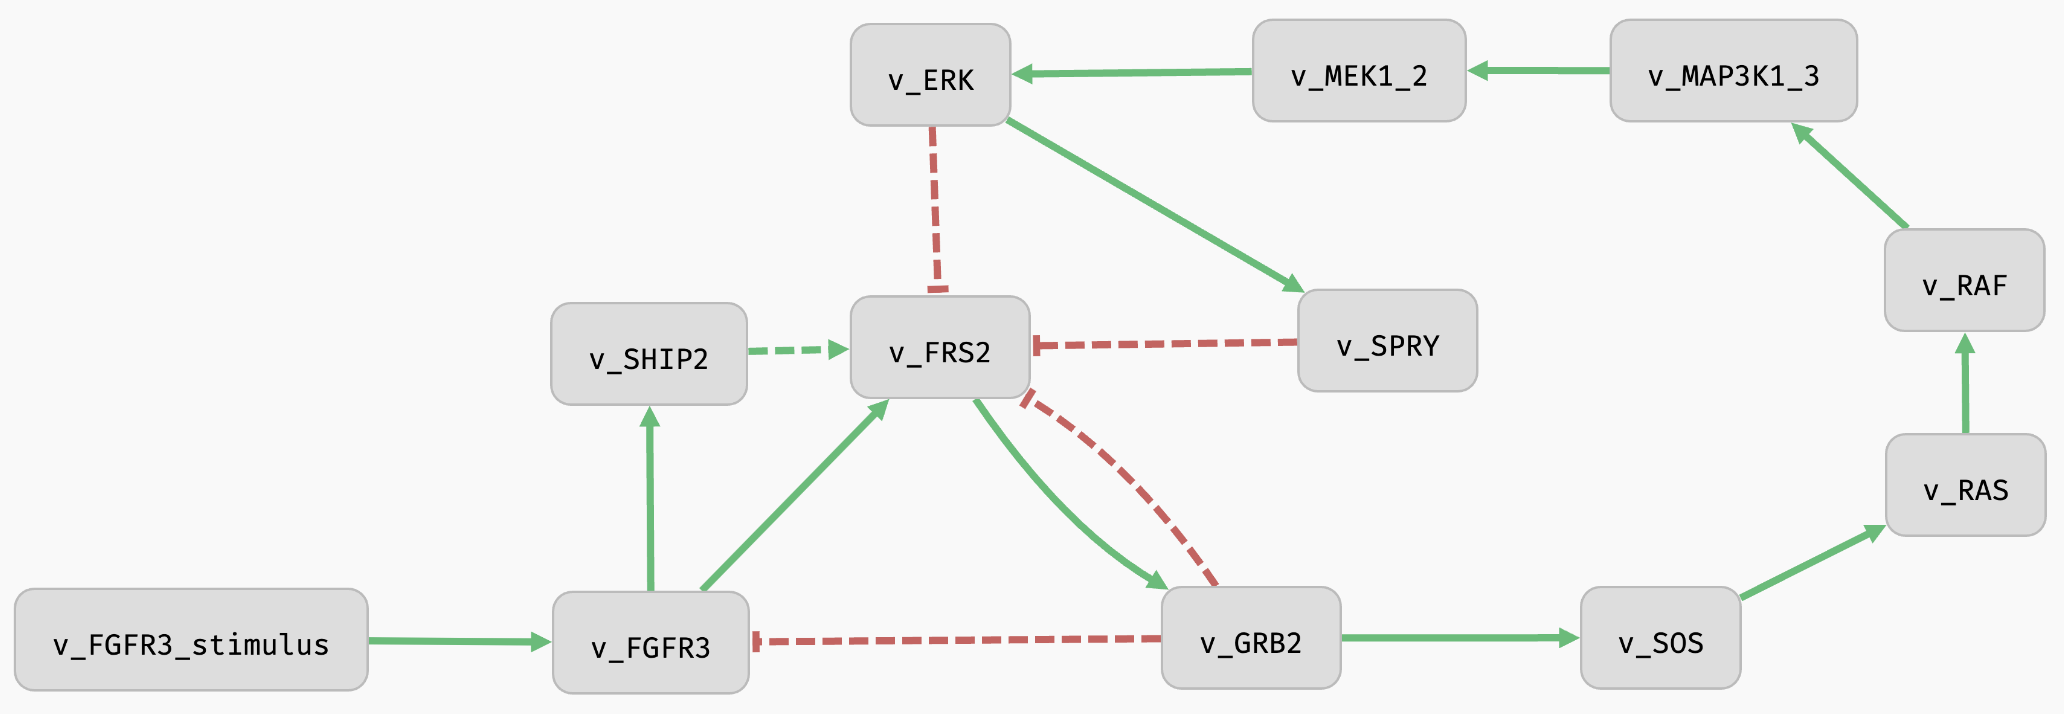
\includegraphics[width=\textwidth]{Figures/fgfr3_isolated.png}
  \caption{\textbf{An isolated FGFR3 pathway model.} The model consists of 12 variables and 16 regulatory interactions. The variables \var{FRS2} and \var{FGFR3}, are partially specified. The positive regulations are depicted in green color while negative regulations are red. The lines which are dashed represent regulations which are not required to be essential in the model interpretations. The model serves as an example for demonstrating the capabilities of our method.}
  \label{fig:fgfr3_isolated}
  \end{minipage}
  }
\end{figure}

Based on our previous research\cite{HSB}, we consider a minimalistic model representing an abstracted form of FGFR3-MAPK signaling pathway, focusing on the interactions among FGFR3, FRS2, SHIP2 and ERK proteins~\cite{Barnat2017}. The model is encoded as a PSBN consisting of 12 variables and 16 regulatory interactions. The model contains one input -- \var{FGFR3\_stimulus}, which is considered implicitly set to true to simulate constitutive activation of the pathway via suitable FGF ligands. This stimulus can be however disabled (perturbed to the value 0) with the phenotype control. The update logics of \var{FGFR3} and \var{FRS2} is partially specified reflecting the fact that the combined effect of variables regulating their activity as well as the presence of particular regulations is not well understood~\cite{Krejci2012,Santhana2023}. 

The dynamics of the final protein component ERK closing the isolated pathway forms the (model) phenotype. In particular, we consider three protein-level phenotypes targeting ERK activity: \var{ERK} stabilization, \var{ERK} avoidance, and \var{ERK} oscillation. Due to the introduced uncertainty, the FGFR3 model has 888 possible interpretations. 

%Using the following observations found in literature we perform control-guided model refinement (as depicted in \autoref{fig:control_workflow}) to exclude biologically inconsistent interpretations of the \PBN{}. Our hypotheses are based on the experimental evidence established with \emph{chondrocyte} cells. 

% \begin{enumerate}
%   \item Oscillation of ERK activity can be observed in some settings \cite{Raina2022}.
%   \item FGF stimulus must be present for ERK activation -- the presence of FGF ligands bond to FGFR3 is \emph{de facto} necessary for FGFR3 activation which in case of the isolated mechanism implies the activation of ERK \cite{Krejci2012}.
%   \item SHIP2 knock-out causes ERK activity to be down-regulated but not suppressed completely \cite{Fafilek2018}.
% \end{enumerate}

% We use these observations as accepted prior knowledge to reduce the number of admissible interpretations of the \PBN{}.

\begin{table}[]
\caption{\textbf{FGFR3 pathway model update functions.} The table shows the update functions of the FGFR3 pathway model. The variables \var{FGFR3} and \var{FRS2} are partially specified, while the rest of the variables are fully specified. The function symbols $f$, $g$ and $h$ are unary function symbols, while $\land$ and $\lor$ are binary logical operators.}
\centering
\begin{tabular}{ll}
\hline
\textbf{Variable}   & \textbf{Function}                                         \\
\hline
\var{FGFR3}      & $f(\var{FGFR3\_stimulus}, \var{GRB2})$                          \\
\var{GRB2}       & \var{FRS2}                                             \\
\var{FRS2}       & $\var{FGFR3} \land g(\var{ERK}, \var{GRB2}, \var{SPRY}) \lor (\var{FGFR3} \land h(\var{SHIP2}))$ \\
\var{ERK}        & \var{MEK1\_2}                                           \\
\var{SHIP2}      & \var{FGFR3}                                            \\
\var{SPRY}       & \var{ERK}                                              \\
\var{SOS}        & \var{GRB2}                                             \\
\var{RAS}        & \var{SOS}                                              \\
\var{RAF}        & \var{RAS}                                              \\
\var{MAP3K1\_3}  & \var{RAF}                                              \\
\var{MEK1\_2}    & \var{MAP3K1\_3}  \\
\hline
\end{tabular}
\label{tab:small_mapk_funs}
\end{table}

\begin{table}[ht!]
  \small
  \caption{\textbf{Phenotype control of the isolated FGFR3 pathway model.} The table shows the perturbations that control the model towards the ERK stabilization, avoidance and oscillation phenotypes. The symbol $\emptyset$ denotes an absence of perturbations. The robustness of each perturbation is of all interpretation of the original model is shown in the third column.}
  \centering
  \resizebox{\textwidth}{!}{
  \begin{tabular}{lll}
    \hline
    \textbf{Phenotype}                 & \textbf{Perturbation}                                                                                            & $\robustness$  \\ \hline
    \multirow{6}{*}{ERK stabilization} & \begin{tabular}[c]{@{}l@{}}\var{FRS2}=1, \var{GRB2}=1, \var{MAPK3K1\_3}=1, \var{MEK1\_2}=1, \\ \var{RAF}=1, \var{RAS}=1, \var{SOS}=1\end{tabular}          & 1                 \\[2.1ex]
                                      & \var{FGFR3}=1                                                                                                          & 0.94                \\[1ex]

                                       & \var{SPRY}=0                                                                                                          & 0.637                \\[1ex]
                                       & \O, \var{SHIP2}=1, \var{SPRY}=1                                                                                                     & 0.626           \\
                                       & \var{SHIP2}=0                                                                                    & 0.583             \\ \midrule
    \multirow{4}{*}{ERK avoidance}     & \begin{tabular}[c]{@{}l@{}}\var{FGFR3}=0, \var{FRS2}=0, \var{GRB2}=0, \var{MAPK3K1\_3}=0,\\ \var{MEK1\_2}=1, \var{RAF}=0, \var{RAS}=0, \var{SOS}=0\end{tabular} & 1             \\[2ex]
                                       & \var{FGFR3\_st.}=0                                                                                                & 0.667     \\[1ex]
                                       & \var{SPRY}=1                                                                                                           & 0.017                 \\ \midrule
    \multirow{8}{*}{ERK oscillation}   & \var{SHIP2}=0                                                                                                          & 0.41                \\[1ex]
                                       & \O, \var{SHIP2}=1                                                             & 0.374           \\[1ex]
                                       & \var{SPRY}=0                                                             & 0.363        \\[1ex]
                                       & \var{SPRY}=1                                                            & 0.357          \\[1ex] 
                                       & \var{FGFR3}=1                                                            & 0.061        \\[1ex] 
                                       & \var{FGFR3\_stimulus}=0                                                            & 0.333     \\[1ex] \midrule

    \end{tabular}}
  \label{tab:fgfr3_isolated}
  \end{table}



Let us we observe the non-perturbed behavior -- the ``natural'' phenotypes of the model. After running a simple algorithm for searching the attractors supported in AEON.py, we learn that the unperturbed model stabilizes in 2 types of attractors -- \var{ERK} stabilization (556 interpretations) and \var{ERK} oscillation (332 interpretations). The \var{ERK} avoidance phenotype was not observed in the non-perturbed version of the model. This is due to the presence of the \var{FGFR3\_stimulus} which we have set to true for our experiments. The stimulus transitively activates \var{ERK} via \var{FGFR3}, \var{FRS2} and other transitive variables.

\paragraph{Initial perturbation screening}

Next, we computed the phenotype control for all three considered phenotypes. The results are summarized in Table~\ref{tab:fgfr3_isolated}. Due to the small size of the model, we list only perturbations up to size one, since perturbations of bigger size did not achieve better results; not even in case of oscillation, where no perturbation has 100\% robustness. Even when perturbations of all sizes were computed, no perturbation achieved better robustness towards oscillation phenotype than \var{SHIP2}=0. This might be due to the incomplete model design, which we will discuss later.

\begin{figure}[ht!]
\captionsetup[subfigure]{justification=centering}
\checkoddpage
\edef\side{\ifoddpage l\else r\fi}
\makebox[\textwidth][\side]{% 
	\begin{minipage}{\fullwidth}
  \centering
  \subfloat[ERK stabilization.]{
    \label{subfig:true_upset}
    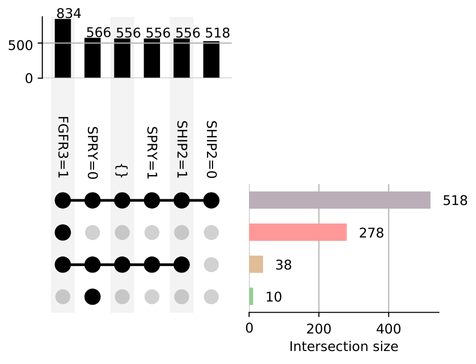
\includegraphics[width=0.5\textwidth]{Figures/fgfr3_isolated_exp/erk_true_upset_colors.png}
  }\hfill
  \subfloat[ERK stabilization - Venn diagram.]{
    \label{subfig:true_venn}
    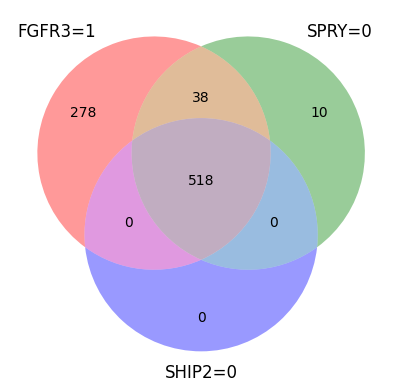
\includegraphics[width=0.4\textwidth]{Figures/fgfr3_isolated_exp/erk_true_venn.png}
  }\hfill
  \subfloat[ERK avoidance.]{
    \label{subfig:false_upset}
    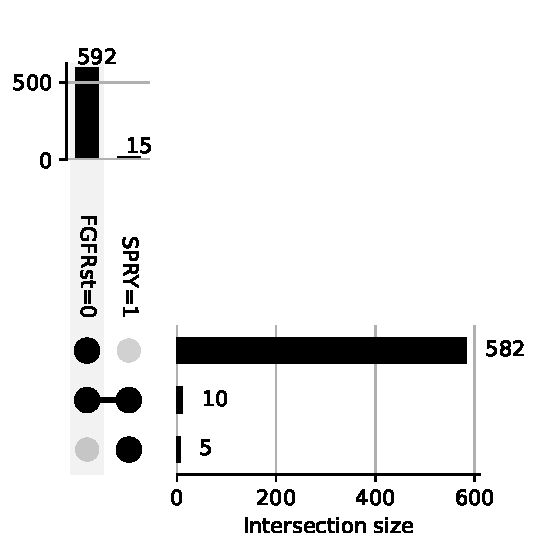
\includegraphics[width=0.35\textwidth]{Figures/fgfr3_isolated_exp/small_fgfr3_isolated_erk_avoidance_upset_full.pdf}
  }
  \subfloat[ERK oscillation.]{
    \label{subfig:oscillation_upset}
    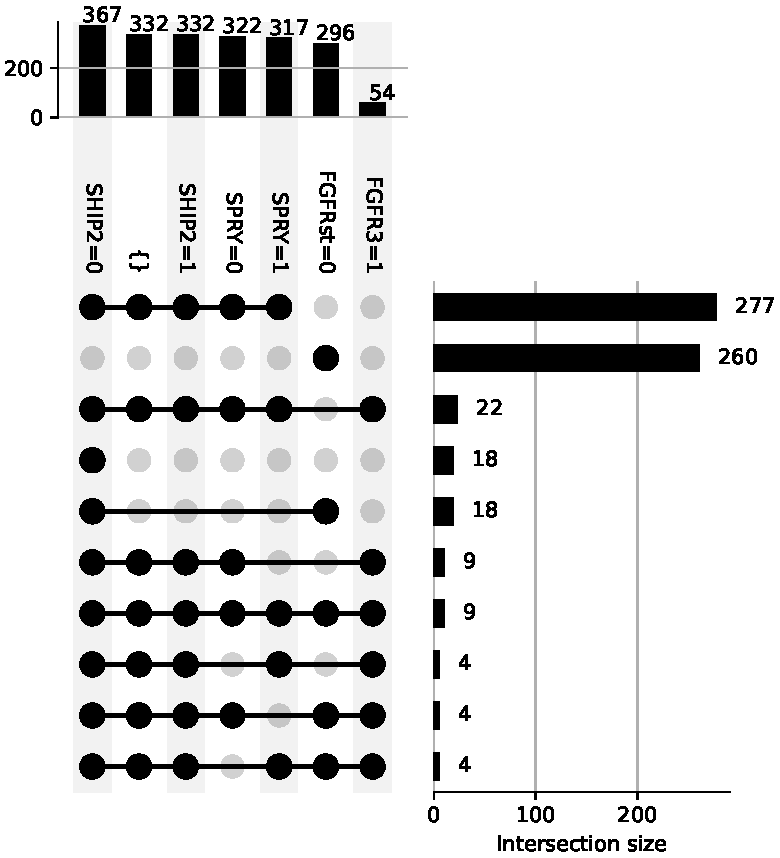
\includegraphics[width=0.6\textwidth]{Figures/fgfr3_isolated_exp/small_fgfr3_isolated_erk_oscillation_compact.pdf}
  }
  \caption{\textbf{Data informing selection of knockout and over-expression experiments to refine model uncertainty.} \autoref{subfig:true_upset},\autoref{subfig:false_upset}, and \autoref{subfig:oscillation_upset} use UpSet plots~\cite{Lex2014} to represent intersections between sets of interpretations controlled by particular perturbations into ERK stabilization, avoidance and oscillation. \autoref{subfig:true_venn} then represent intersections between controlled interpretations by perturbation candidates selected from \autoref{subfig:true_upset}.}
  \label{fig:fgfr3_isolated_exp}
  \end{minipage}
  }
\end{figure}


We can also notice, that perturbation of the same variable to both true and false may lead to the same phenotype (e.g. \var{SPRY} in case of oscillation). Similarly, the same perturbations can lead to multiple phenotypes (e.g. \var{SHIP2}=1). This is because in these cases the partially specified functions have a greater influence on the network dynamics, than the perturbation itself -- thus, another plausible explanation is, that the network behaves the same way as without any perturbations. In case, this is not expected behavior, this can be seen as a flaw introduced in some interpretations of the model which should be therefore refuted.

To probe further all the unexpected model behavior we use the framework of perturbation experiments. First, we need to observe which perturbations yield the most differing results in terms of controlled interpretations. To do this, we can depict intersections of the interpretation sets controlled by various perturbations with a robustness lesser than 100\%. The results of such an analysis are displayed in Fig.~\ref{fig:fgfr3_isolated_exp}. We use Upset plots for the visualization~\cite{Lex2014}.

We can see, that \var{ERK} avoidance case (Subfig.~\ref{subfig:false_upset}) gives us very straightforward answer of which perturbations should be selected, since there are only two perturbations (\var{FGFR3\_stimulus}=0 and \var{SPRY}=1) covering unique sets of interpretations (the same can be seen from Table~\ref{tab:fgfr3_isolated}). 

The case of \var{ERK} stabilization (Subfig.~\ref{subfig:true_upset}) is a bit more complicated, as there are multiple perturbations that could be selected. Nonetheless, we can notice, that \var{SPRY}=0 and \var{FGFR3}=1 should be selected, since they cover some unique set of interpretations. Similarly, \var{SHIP2}=0 should be selected, because it is missing some interpretations covered by all other perturbations (i.e, it is unique by interpretations which it is \emph{not} covering). Finally, as we can see in the Subfig.~\ref{subfig:true_venn}, these three perturbations are sufficient to cover all subset cases of the \var{ERK} stabilization.

Last but not least, we consider phenotype control to oscillating \var{ERK} (Subfig.~\ref{subfig:oscillation_upset}). We can notice, that we have already selected all other perturbations to be in the perturbation experiments apart from an empty perturbation and \var{SHIP2}=1. However, these two perturbations have exactly the same behavior, and thus we can arbitrarily choose any of them -- we choose an empty perturbation (since it would be expected to be easier to implement). The results of the perturbation experiments are summarized in Table~\ref{tab:fgfr3_isolated_interpretations}.

\begin{table}[htb!]
  \caption{\textbf{Information gain of interpretation features.} The table shows information gain of the three best performing features (four in case of exact match) per each labelling (assessment whether a perturbation is working). The features highlighted in blue were selected to be considered in the next experiment.}
  \centering
  \resizebox{\textwidth}{!}{
  \begin{tabular}{clc}
  \hline
  \textbf{Perturbation} & \textbf{Feature} & \textbf{NMIS} \\ \hline
  \multirow{3}{*}{$\emptyset$} & \textcolor{blue}{$\exists$\var{SPRY}$\rightarrow$\var{FRS2} ($\feature_1$)} & 0.364 \\
  & \textcolor{blue}{$\forall$\var{SPRY}$\rightarrow$\var{FRS2} ($\feature_2$)} & 0.279 \\
  & $\exists$\var{SPRY}$\rightarrow$\var{SHIP2} & 0.279 \\
  \midrule

  \multirow{3}{*}{\var{SPRY}=0} & \textcolor{blue}{$\exists$\var{FGFR3} = \var{FGFR3\_stimulus} $\land$ $\neg$\var{GRB2} ($\feature_3$)} & 0.529 \\
  & \textcolor{blue}{$\forall$\var{GRB2}$\rightarrow$\var{FGFR3} ($\feature_4$)} & 0.293 \\
  & $\forall$\var{FRS2} = \var{FGFR\_stimulus} & 0.293 \\
  \midrule

  \multirow{3}{*}{\var{SHIP2}=0}  & \textcolor{blue}{$\forall$\var{SPRY}$\rightarrow$\var{FRS2} ($\feature_2$)} & 0.855 \\
   & \textcolor{blue}{$\forall$\var{FRS2} = \var{FGFR3} $\land$ \var{SHIP2} ($\feature_5$)} & 0.735 \\ 
  & $\exists.$\var{FRS2} = \var{FGFR3} $\land$ \var{SHIP2} & 0.735 \\ 
   \midrule

  \multirow{2}{*}{\var{FGFR3\_stimulus}=0} & \textcolor{blue}{$\forall$\var{FGFR3} = $\neg$\var{GRB2} $\lor$ \var{FGFR3\_stimulus} ($\feature_6$)} & 1.000 \\
   & $\exists$\var{FGFR3} = $\neg$\var{GRB2} $\lor$ \var{FGFR3\_stimulus} & 1.000 \\ 
   \midrule

  \multirow{2}{*}{\var{SPRY}=1} & \textcolor{blue}{$\exists$\var{SPRY}$\rightarrow$\var{FRS2} ($\feature_1$)} & 0.485 \\
    & \textcolor{blue}{$\exists$\var{FRS2} = \var{FGFR3} $\land$ $\neg$\var{SPRY} ($\feature_7$)} & 0.437 \\ 
    \midrule

  \multirow{4}{*}{\var{FGFR3}=1} & \textcolor{blue}{$\forall$\var{SHIP2}$\rightarrow$\var{FRS2} ($\feature_8$)} & 0.562 \\
  & \textcolor{blue}{$\exists$\var{SPRY}$\rightarrow$\var{FRS2} ($\feature_1$)} & 0.562 \\
    & \textcolor{blue}{$\forall$\var{SPRY}$\rightarrow$\var{FRS2} ($\feature_2$)} & 0.442 \\ 
    & $\exists$\var{SHIP2}$\rightarrow$\var{FRS2} & 0.442 \\ \midrule
  \end{tabular}
  }
  \label{tab:fgfr3_isolated_features}
  \end{table}

Before diving into the results of the interpretation split and model behavior under differing perturbations we might first pose the question: ``Why a perturbation works for some particular set of interpretations and not for others?'' in order to better explain the observed model behavior. To inquire that, we can look into a set of common \emph{features} of the labelled interpretations, where \emph{label} is an assessment which phenotype (ERK avoidance, activation, or oscillation) is manifested by a given interpretation.

% \begin{table}[b!]
%   \footnotesize
%   \setlength{\tabcolsep}{4pt}
% \checkoddpage
% \edef\side{\ifoddpage l\else r\fi}
% \makebox[\textwidth][\side]{% 
% \begin{minipage}[t]{\fullwidth}
%   \caption{\textbf{Behavior of isolated FGFR3 pathway interpretations under perturbations.} Each row reflects interpretations sharing a particular behaviour pattern (ERK exhibiting specific phenotypes under considered perturbation experiments). The first column displays a row index while the second column indicates how many interpretations exhibit the displayed behavior pattern. The second column describes ERK phenotypes achieved under the listed knockout/over-expression experiments, in particular: no perturbation (\O), \var{SPRY}=0 ($\perturbation_1$), \var{SHIP2}=0 ($\perturbation_2$), \var{FGFR3\_stimulus}=0 ($\perturbation_3$), \var{SPRY}=1 ($\perturbation_4$), and \var{FGFR3}=1 ($\perturbation_5$). The values denote the phenotypes: \var{ERK} stabilization (1), avoidance (0), or oscillation (\oscil). The last column represents relevant model features, i.e., the fact whether all corresponding interpretations fullfill them: $\exists$\var{SPRY}$\rightarrow$\var{FRS2} ($F_1$), $\forall$\var{SPRY}$\rightarrow$\var{FRS2} ($F_2$), $\exists\var{FGFR3} = \var{FGFR3\_stim.} \land \neg $\var{GRB2} ($F_3$), \var{GRB2}$\rightarrow$\var{FGFR3} ($F_4$), $\forall$\var{FRS2} = \var{FGFR3} $\land$ \var{SHIP2} ($F_5$), $\forall$\var{FGFR3} = $\neg$\var{GRB2} $\lor$ \var{FGFR3\_stimulus} ($F_6$), $\forall$\var{FRS2} = \var{FGFR3} $\land$ $\neg$\var{SPRY} ($F_7$), and $\forall$\var{SHIP2}$\rightarrow$\var{FRS2} ($F_8$). Rows highlighted in \sethlcolor{lightgray}\hl{gray} allow non-trivial \var{ERK} activity even with \var{FGFR3\_stimulus=0}, violating our first assumption. The three \sethlcolor{green!30}\hl{green} rows are the rows which satisfy both of our control-guided assumptions.}
%     \centering
%   \begin{tabular}{|r|l|cccccc|cccccccc|}
% \hline
%      &    & \multicolumn{6}{c|}{ERK under perturbation}                 &  \multicolumn{8}{c|}{Features of $\interpretationSet$} \\ 
%   \# & $\mid\interpretationSet\mid$ & \O & $\perturbation_1$ & $\perturbation_2$ & $\perturbation_3$ & $\perturbation_4$ & $\perturbation_5$ & $\feature_1$ & $\feature_2$ & $\feature_3$ & $\feature_4$ & $\feature_5$ & $\feature_6$ & $\feature_7$ & $\feature_8$\\[1ex] \hline 
%   1  & 277 & \oscil & \oscil & \oscil & 0 & \oscil      & 1      & 0 & 1 & 1 & 1 & 0 & 0 & 0 & 1 \\
%   2  & 259 & 1      & 1      & 1      & 0      & 1      & 1      & 0 & 0 & 0 & 0 & 0 & 0 & 0 & 0 \\
%   \rowcolor{lightgray}  
%   3  & 259 & 1      & 1      & 1      & \oscil     & 1 & 1      & 0 & 0 & 0 & 1 & 0 & 1 & 0 & 0\\
%   4  & 22  & \oscil & \oscil & \oscil & 0 & \oscil      & \oscil & 0 & 1 & 1 & 1 & 0 & 0 & 0 & 0 \\
%   \rowcolor{green!30}
%   5  & 18  & 1      & 1      & \oscil      & 0 & 1      & 1      & 0 & 1 & 0 & 0 & 0 & 0 & 0 & 1 \\
%   \rowcolor{lightgray}  
%   6   & 18  & 1      & 1      & \oscil    & \oscil    & 1 & 1      & 0 & 1 & 0 & 1 & 0 & 1 & 0 & 1 \\
%   7  & 9   & \oscil & \oscil & \oscil     & 0 & 0      & \oscil & 1 & 1 & 1 & 1 & 0 & 0 & 1 & 0 \\
%    \rowcolor{lightgray}  
%   8  & 9   & \oscil & \oscil & \oscil & \oscil & \oscil & \oscil & 0 & 1 & 0 & 1 & 0 & 1 & 0 & 0 \\
%   9  & 4   & \oscil & 1      & \oscil & 0 & \oscil     & \oscil  & 1 & 1 & 0 & 0 & 0 & 0 & 0 & 0 \\
%    \rowcolor{lightgray}  
%   10 & 4   & \oscil & 1      & \oscil & \oscil & \oscil & \oscil & 1 & 1 & 0 & 1 & 0 & 1 & 0 & 0 \\
%    \rowcolor{lightgray}  
%   11 & 4   & \oscil & \oscil & \oscil  & \oscil & 0 & \oscil & 1 & 1 & 0 & 1 & 0 & 1 & 0 & 0 \\
%     \rowcolor{green!30}
%   12 & 1   & \oscil & \oscil  & 0  & 0 & \oscil     & 0 & 0 & 0 & 1 & 1 & 1 & 0 & 0 & 1 \\
%   \rowcolor{lightgray}  
%   13 & 1   & \oscil & 1      & \oscil      & \oscil & 0 & \oscil & 1 & 1 & 0 & 1 & 0 & 1 & 1 & 0 \\
%   \rowcolor{green!30}
%   14 & 1   & 1      & 1      & 0      & 0      & 1      & 1      & 0 & 0 & 0 & 0 & 1 & 0 & 0 & 1\\
%   \rowcolor{lightgray}  
%   15 & 1   & 1  &  1 &  0      & \oscil      & 1        & 1      & 0 & 0 & 0 & 1 & 1 & 1 & 0 & 1 \\
%   16 & 1   & \oscil & 1 & \oscil & 0      & 0      & \oscil     & 1 & 1 & 0 & 0 & 0 & 0 & 1 & 0 \\
%   \hline
%   \end{tabular}
%   \label{tab:fgfr3_isolated_interpretations}
%   \end{minipage}}
%   \end{table}

\paragraph{Feature-based perturbation selection}

\begin{table}
	\caption{\textbf{Mutual information score of interpretation features.} NMIS of the three best performing features (four in case of equal scores) per each labeling (assessment of phenotypes under perturbation). We then consider only non-redundant features (e.g., an existential feature is redundant if its universal variant has an equal or higher NMIS); these are assigned names $\feature_1, \ldots, \feature_8$.}
	\centering
	\vspace{4pt}
	\begin{tabular}{rlrlc}
		\hline
		&\textbf{Pert.} & & \textbf{Feature} & \textbf{NMIS} \\ \hline
		&\multirow{3}{*}{\O} & $\feature_1$ & $\forall$\var{SPRY}$\rightarrow$\var{FRS2} & 0.364 \\
		&& $\feature_2$ & $\exists$\var{SPRY}$\rightarrow$\var{FRS2} & 0.279 \\
		&& & $\forall$\var{SPRY}$\rightarrow$\var{SHIP2} & 0.279 \\
		\midrule
		
		\multirow{3}{*}{$Q_1$} & \multirow{3}{*}{\texttt{SPRY=0}} & $\feature_3$ & $\exists$\var{FGFR3} = \var{FGFR3\_st.} $\land$ $\neg$\var{GRB2} & 0.529 \\
		&& $\feature_4$ & $\exists$\var{GRB2}$\rightarrow$\var{FGFR3} & 0.293 \\
		&& & $\exists$\var{FRS2} = \var{FGFR3\_st.} & 0.293 \\
		\midrule
		
		\multirow{3}{*}{$Q_2$} &\multirow{3}{*}{\texttt{SHIP2=0}} & $\feature_2$ & $\exists$\var{SPRY}$\rightarrow$\var{FRS2} & 0.855 \\
		&& $\feature_5$ & $\forall$\var{FRS2} = \var{FGFR3} $\land$ \var{SHIP2} & 0.735 \\ 
		&& & $\exists$\var{FRS2} = \var{FGFR3} $\land$ \var{SHIP2} & 0.735 \\ 
		\midrule
		
		\multirow{2}{*}{$Q_3$} &\multirow{2}{*}{\texttt{FGFR3\_st.=0}} & $\feature_6$ & $\forall$\var{FGFR3} = $\neg$\var{GRB2} $\lor$ \var{FGFR3\_st.} & 1.000 \\ 
		&&& $\exists$\var{FGFR3} = $\neg$\var{GRB2} $\lor$ \var{FGFR3\_st.} & 1.000 \\  
		\midrule
		
		\multirow{2}{*}{$Q_4$} &\multirow{2}{*}{\texttt{SPRY=1}} & $\feature_1$ & $\forall$\var{SPRY}$\rightarrow$\var{FRS2} & 0.485 \\
		&& $\feature_7$ & $\exists$\var{FRS2} = \var{FGFR3} $\land$ $\neg$\var{SPRY} & 0.437 \\ 
		\midrule
		
		\multirow{4}{*}{$Q_5$} &\multirow{4}{*}{\texttt{FGFR3=1}} & $\feature_8$& $\exists$\var{SHIP2}$\rightarrow$\var{FRS2} & 0.562 \\
		&& $\feature_1$ & $\forall$\var{SPRY}$\rightarrow$\var{FRS2} & 0.562 \\
		&& $\feature_2$ & $\exists$\var{SPRY}$\rightarrow$\var{FRS2} & 0.442 \\ 
		&&& $\forall$\var{SHIP2}$\rightarrow$\var{FRS2} & 0.442 \\ \midrule
	\end{tabular}
	\label{tab:fgfr3_isolated_features}
	\vspace{-8pt}
\end{table}

To select the most relevant perturbations out of the 5 remaining, 
we consider which features of the PSBN best explain the perturbation outcomes. 
First, the candidate perturbations classify the 888 PSBN interpretations into 
16 equivalence classes based on the phenotypes of the perturbed model 
(i.e., \var{ERK} stabilisation, avoidance, or oscillation). 
We then assign each class a collection of feature values, 
corresponding to concrete properties of the candidate BNs. 
Each such feature can be either held universally by \emph{all} 
members of the class (denoted $\forall$), or existentially (denoted $\exists$) 
by \emph{some} members of the class (naturally, if a feature is universally held in a class, 
it is by definition also held existentially). 
Here, the specific set of features consists of (a) essentiality of the five uncertain regulations; 
(b) individual interpretations of the network's partially unknown update functions.

For every perturbation-feature pair, 
we compute the NMIS between the perturbation outcome and the feature. 
This score indicates which features correctly predict phenotypes of the perturbed model. 
The results of this analysis are presented in Table~\ref{tab:fgfr3_isolated_features}. 
Here, the most prominent perturbation is \var{FGFR3\_stimulus=0}, where the phenotypes are
 perfectly predicted by the choice of update function in \var{FGFR3} (NMIS is $1.0$). 
The second most prominent feature is the regulation 
 $\var{SPRY} \to \var{FRS2}$ when subject to perturbation \var{SHIP2=0} (NMIS is $0.855$). 
 Both \var{SHIP2} and \var{SPRY} are considered uncertain regulators of \var{FRS2} in our PSBN, 
 which is the second variable with a partially specified update function in our model. 
 Consequently, this indicates that the interplay of these two regulators is the most 
 important for determining the update function of \var{FRS2}.

\sethlcolor{lightgray}

\begin{table}
	\caption{\textbf{Behavior of the isolated FGFR3 pathway under perturbations.} Each row corresponds to a class of interpretations characterized by their perturbation response. Here, \# is the row index and $|\interpretationSet|$ is size of the interpretations class. Then, we describe \var{ERK} phenotypes achieved under specific perturbations, as listed in Table~\ref{tab:fgfr3_isolated_features} (phenotypes represent \var{ERK} stabilisation (1), avoidance (0), or oscillation (\oscil)). The last two columns represent selected model features (also listed in Table~\ref{tab:fgfr3_isolated_features}) representing guaranteed presence of regulations, and guaranteed update function specification. Rows highlighted in \sethlcolor{lightgray}\hl{gray} allow non-trivial \var{ERK} activity even with \var{FGFR3\_st.=0}, violating our first assumption. The three \sethlcolor{green!30}\hl{green} rows are the rows which satisfy both of our control-guided assumptions.}
	\centering
	\vspace{4pt}
	\scalebox{0.9}{\footnotesize
		\begin{tabular}{|r|l|cccccc|ccc|cc|}
			\hline
			&    & \multicolumn{6}{c|}{\var{ERK} under perturbation}                 &  \multicolumn{3}{c|}{$\exists\var{A} \rightarrow \var{B}$} & \multicolumn{2}{c|}{$\forall\var{A} = \var{ex.}$} \\ 
			\# & $\mid\interpretationSet\mid$ & \O & $\perturbation_1$ & $\perturbation_2$ & $\perturbation_3$ & $\perturbation_4$ & $\perturbation_5$ & $\feature_2$ & $\feature_4$ & $\feature_8$ & $\feature_5$ & $\feature_6$ \\ \hline 
			1  & 277 & \oscil & \oscil & \oscil & 0 & \oscil      & 1      & 1 & 1 & 1 & 0 & 0\\
			2  & 259 & 1      & 1      & 1      & 0      & 1      & 1      & 0 & 0 & 0 & 0 & 0 \\
			\rowcolor{lightgray}
			3  & 259 & 1      & 1      & 1      & \oscil     & 1 & 1      & 0 & 1 & 0 & 0 & 1 \\
			4  & 22  & \oscil & \oscil & \oscil & 0 & \oscil      & \oscil & 1 & 1 & 0 & 0 & 0 \\
			\rowcolor{green!30}
			5  & 18  & 1      & 1      & \oscil      & 0 & 1      & 1      & 1  & 0 & 1 & 0 & 0 \\
			\rowcolor{lightgray}
			6   & 18  & 1      & 1      & \oscil    & \oscil    & 1 & 1      & 1  & 1 & 1 & 0 & 1 \\
			7  & 9   & \oscil & \oscil & \oscil     & 0 & 0      & \oscil & 1 & 1 & 0 & 0 & 0\\
			\rowcolor{lightgray}
			8  & 9   & \oscil & \oscil & \oscil & \oscil & \oscil & \oscil & 1 & 1 & 0 & 0 & 1 \\
			9  & 4   & \oscil & 1      & \oscil & 0 & \oscil     & \oscil  & 1 & 0 & 0 & 0 & 0\\
			\rowcolor{lightgray}
			10 & 4   & \oscil & 1      & \oscil & \oscil & \oscil & \oscil & 1 & 1 & 0 & 0 & 1\\
			\rowcolor{lightgray}
			11 & 4   & \oscil & \oscil & \oscil  & \oscil & 0 & \oscil & 1 & 1 & 0 & 0 & 1\\
			\rowcolor{green!30}
			12 & 1   & \oscil & \oscil  & 0  & 0 & \oscil     & 1 & 0 & 1 & 1 & 1 & 0\\
			\rowcolor{lightgray}
			13 & 1   & \oscil & 1      & \oscil      & \oscil & 0 & \oscil & 1 & 1 & 0 & 0 & 1\\
			\rowcolor{green!30}
			14 & 1   & 1      & 1      & 0      & 0      & 1      & 1      & 0 & 0 & 1 & 1 & 0 \\
			\rowcolor{lightgray}
			15 & 1   & 1  &  1 &  0      & \oscil      & 1        & 1      & 0 & 1 & 1 & 1 & 1 \\
			16 & 1   & \oscil & 1 & \oscil & 0      & 0      & \oscil     & 1 & 0 & 0 & 0 & 0 \\
			\hline
	\end{tabular}}
	\label{tab:fgfr3_isolated_interpretations}
	\vspace{-8pt}
\end{table}

\paragraph{Model refinement}

Based on our results in Table~\ref{tab:fgfr3_isolated_features}, 
we consider \texttt{FGFR3\_stimulus=0} ($Q_3$) and \texttt{SHIP2=0} ($Q_2$) 
to be the most relevant for the identification of a concrete model refinement. 
We performed a literature search to identify plausible experimental results for these 
two most relevant perturbations, leading to the following assumptions: 
First, based on~\cite{KrejciReview2012}, we expect \var{FGFR3\_stimulus} 
to be \emph{necessary} to achieve \var{ERK} stabilisation or oscillation in this isolated model. 
Second, based on~\cite{Fafilek2018}, 
we observe that \var{SHIP2=0} knock-out causes down-regulation of \var{ERK} activity.

To put these assumptions into context, we prepared Table~\ref{tab:fgfr3_isolated_interpretations}, 
which partitions the PSBN interpretations into equivalence classes based on the effects of our five 
chosen perturbations on its phenotypes. Within this table, we can easily identify that only 9 equivalence classes 
(namely 1,2,4,5,7,9,12,14,16) adhere to our first assumption, completely eliminating \var{ERK} activity in response 
to \var{FGFR3\_stimulus=0} ($Q_3$) perturbation. Out of these nine options, the second assumption allows to select rows 
5, 12, and 14, as these are the only cases where the activity of \var{ERK} is plausibly down-regulated compared to 
the unperturbed network in response to \var{SHIP2=0} knock-out ($Q_2$), resulting in 20/888 candidate networks. 

To disambiguate between rows 5, 12, and 14, we would have to quantify the effects observed by~\cite{Fafilek2018}. 
However, based on the fact that~\cite{Fafilek2018} do not report \var{ERK} to be completely inactive, 
we can safely eliminate rows 12 and 14 (where \var{ERK} phenotype drops to 0). 
Furthermore, considering the fact that \var{ERK} is known to oscillate~\citep{Raina2022}, 
we prefer row 5 as the most likely option. 

Interestingly, the 18 networks left in the class at row~5 are completely indistinguishable both in terms of their 
unperturbed phenotypes and their phenotype response to single-variable perturbations. 
More importantly, in these 18 networks, it universally holds that \var{GRB2} does \emph{not} regulate
\var{FGFR3}, but \var{SHIP2} always regulates \var{FRS2} (other regulations remain undetermined). 

% Having a derived set of features and labels, we can compute \emph{normalized mutual information score} (NMIS)~\cite{Kent83} to see which of the features are the most informative per each labelling. We use the following formulas to compute NMIS:

% $$
% IS(X; Y) = \sum_{x, y} P(x, y) \log \frac{P(x, y)}{P(x) P(y)}
% $$
% $$
% H(X) = -\sum_{x} P(x) \log P(x)
% $$
% $$ 
% NMIS(X; Y) = \frac{2 IS(X; Y)}{H(X) H(Y)} 
% $$

% The best performing results of this analysis are shown in \autoref{tab:fgfr3_isolated_features}.
% % The full results can be found in \autoref{appendix:digi_attach}.
 
% For each perturbation in \autoref{tab:grieco_phenotypes_perturbations}, we select two features with the biggest NMIS, unless we obtain complete information (1.0) from a single feature. Therefore, we obtain eight distinct features in total, as can be seen in \autoref{tab:fgfr3_isolated_features}. 

% Next, we can analyse perturbation-phenotype table extended with most representative features in Table~\ref{tab:fgfr3_isolated_interpretations}. We can also demonstrate how analytical observations may easily narrow down sensible interpretations. For example, we may notice, that the rows \#2 and \#14 of the table never lead to the ERK oscillation which can happen only in the absence of cyclic regulations in the partially specified network. This is also reflected by absence of any regulation features for row \#2 as can be seen in detail in the full feature table~\ref{tab:fgfr3_isolated_features}. Even though the row \#14 contains one cycle inducing regulations, it is not sufficient to expose the oscillation behavior for any interpretation, and thus we refute this interpretation as well.

% Another types of interpretations which we refute are the ones where ERK oscillates under \var{FGFR3\_stimulus}=0 (rows \#3, 6, 8, 10, 11, 13, 15). The original intention of the model was, that \var{FGFR3\_stimulus} is required for any \var{ERK} activation. We can also see that exactly the oscillating rows are the ones which contain the feature \var{FGFR3} = $\neg$\var{GRB2} $\lor$ \var{FGFR3\_stimulus}. This shows, that $\neg$\var{GRB2} is sufficient to activate \var{FGFR3} and consequently \var{ERK}, what is in conflict with the intended design.

% Finally, we conducted a literature review in order to identify experimental biology results testing perturbations \var{SHIP2}=0 ($\perturbation_2$) and \var{FGFR3\_stimulus}=0 ($\perturbation_3$), since these perturbations have most prominent efects based on the analytic observations. Studying the recent biological literature related to these signalling components have lead us to declare the following assumptions: 
% First, based on~\cite{Krejci2012}, we expect \var{FGFR3\_stimulus} 
% to be \emph{necessary} to achieve \var{ERK} stabilization or oscillation in this isolated model. 
% Second, based on~\cite{Fafilek2018}, 
% we observe that \var{SHIP2=0} knock-out causes down-regulation of \var{ERK} activity.

% To put the literature-based assumptions into context, we can easily identify that only 9 equivalence classes 
% (namely 1,2,4,5,7,9,12,14,16) adhere to our first assumption, completely eliminating \var{ERK} activity in response 
% to \var{FGFR3\_stimulus=0} ($Q_3$) perturbation. Out of these nine options, the second assumption allows to select rows 
% 5, 12, and 14, as these are the only cases where the activity of \var{ERK} is plausibly down-regulated compared to 
% the unperturbed network in response to \var{SHIP2=0} knock-out ($Q_2$), resulting in 20/888 candidate networks. 

% To disambiguate between rows 5, 12, and 14, we would have to quantify the effects observed by~\cite{Fafilek2018}. 
% However, based on the fact that~\cite{Fafilek2018} do not report \var{ERK} to be completely inactive, 
% we can safely eliminate rows 12 and 14 (where \var{ERK} phenotype drops to 0). 
% Furthermore, considering the fact that \var{ERK} is known to oscillate~\cite{Raina2022}, 
% we prefer row 5 as the most likely option. 

\subsection{Grieco MAPK}

\begin{figure}[ht!]
\checkoddpage
  \edef\side{\ifoddpage l\else r\fi}
  \makebox[\textwidth][\side]{% 
	\begin{minipage}[t]{\fullwidth}
  \centering
  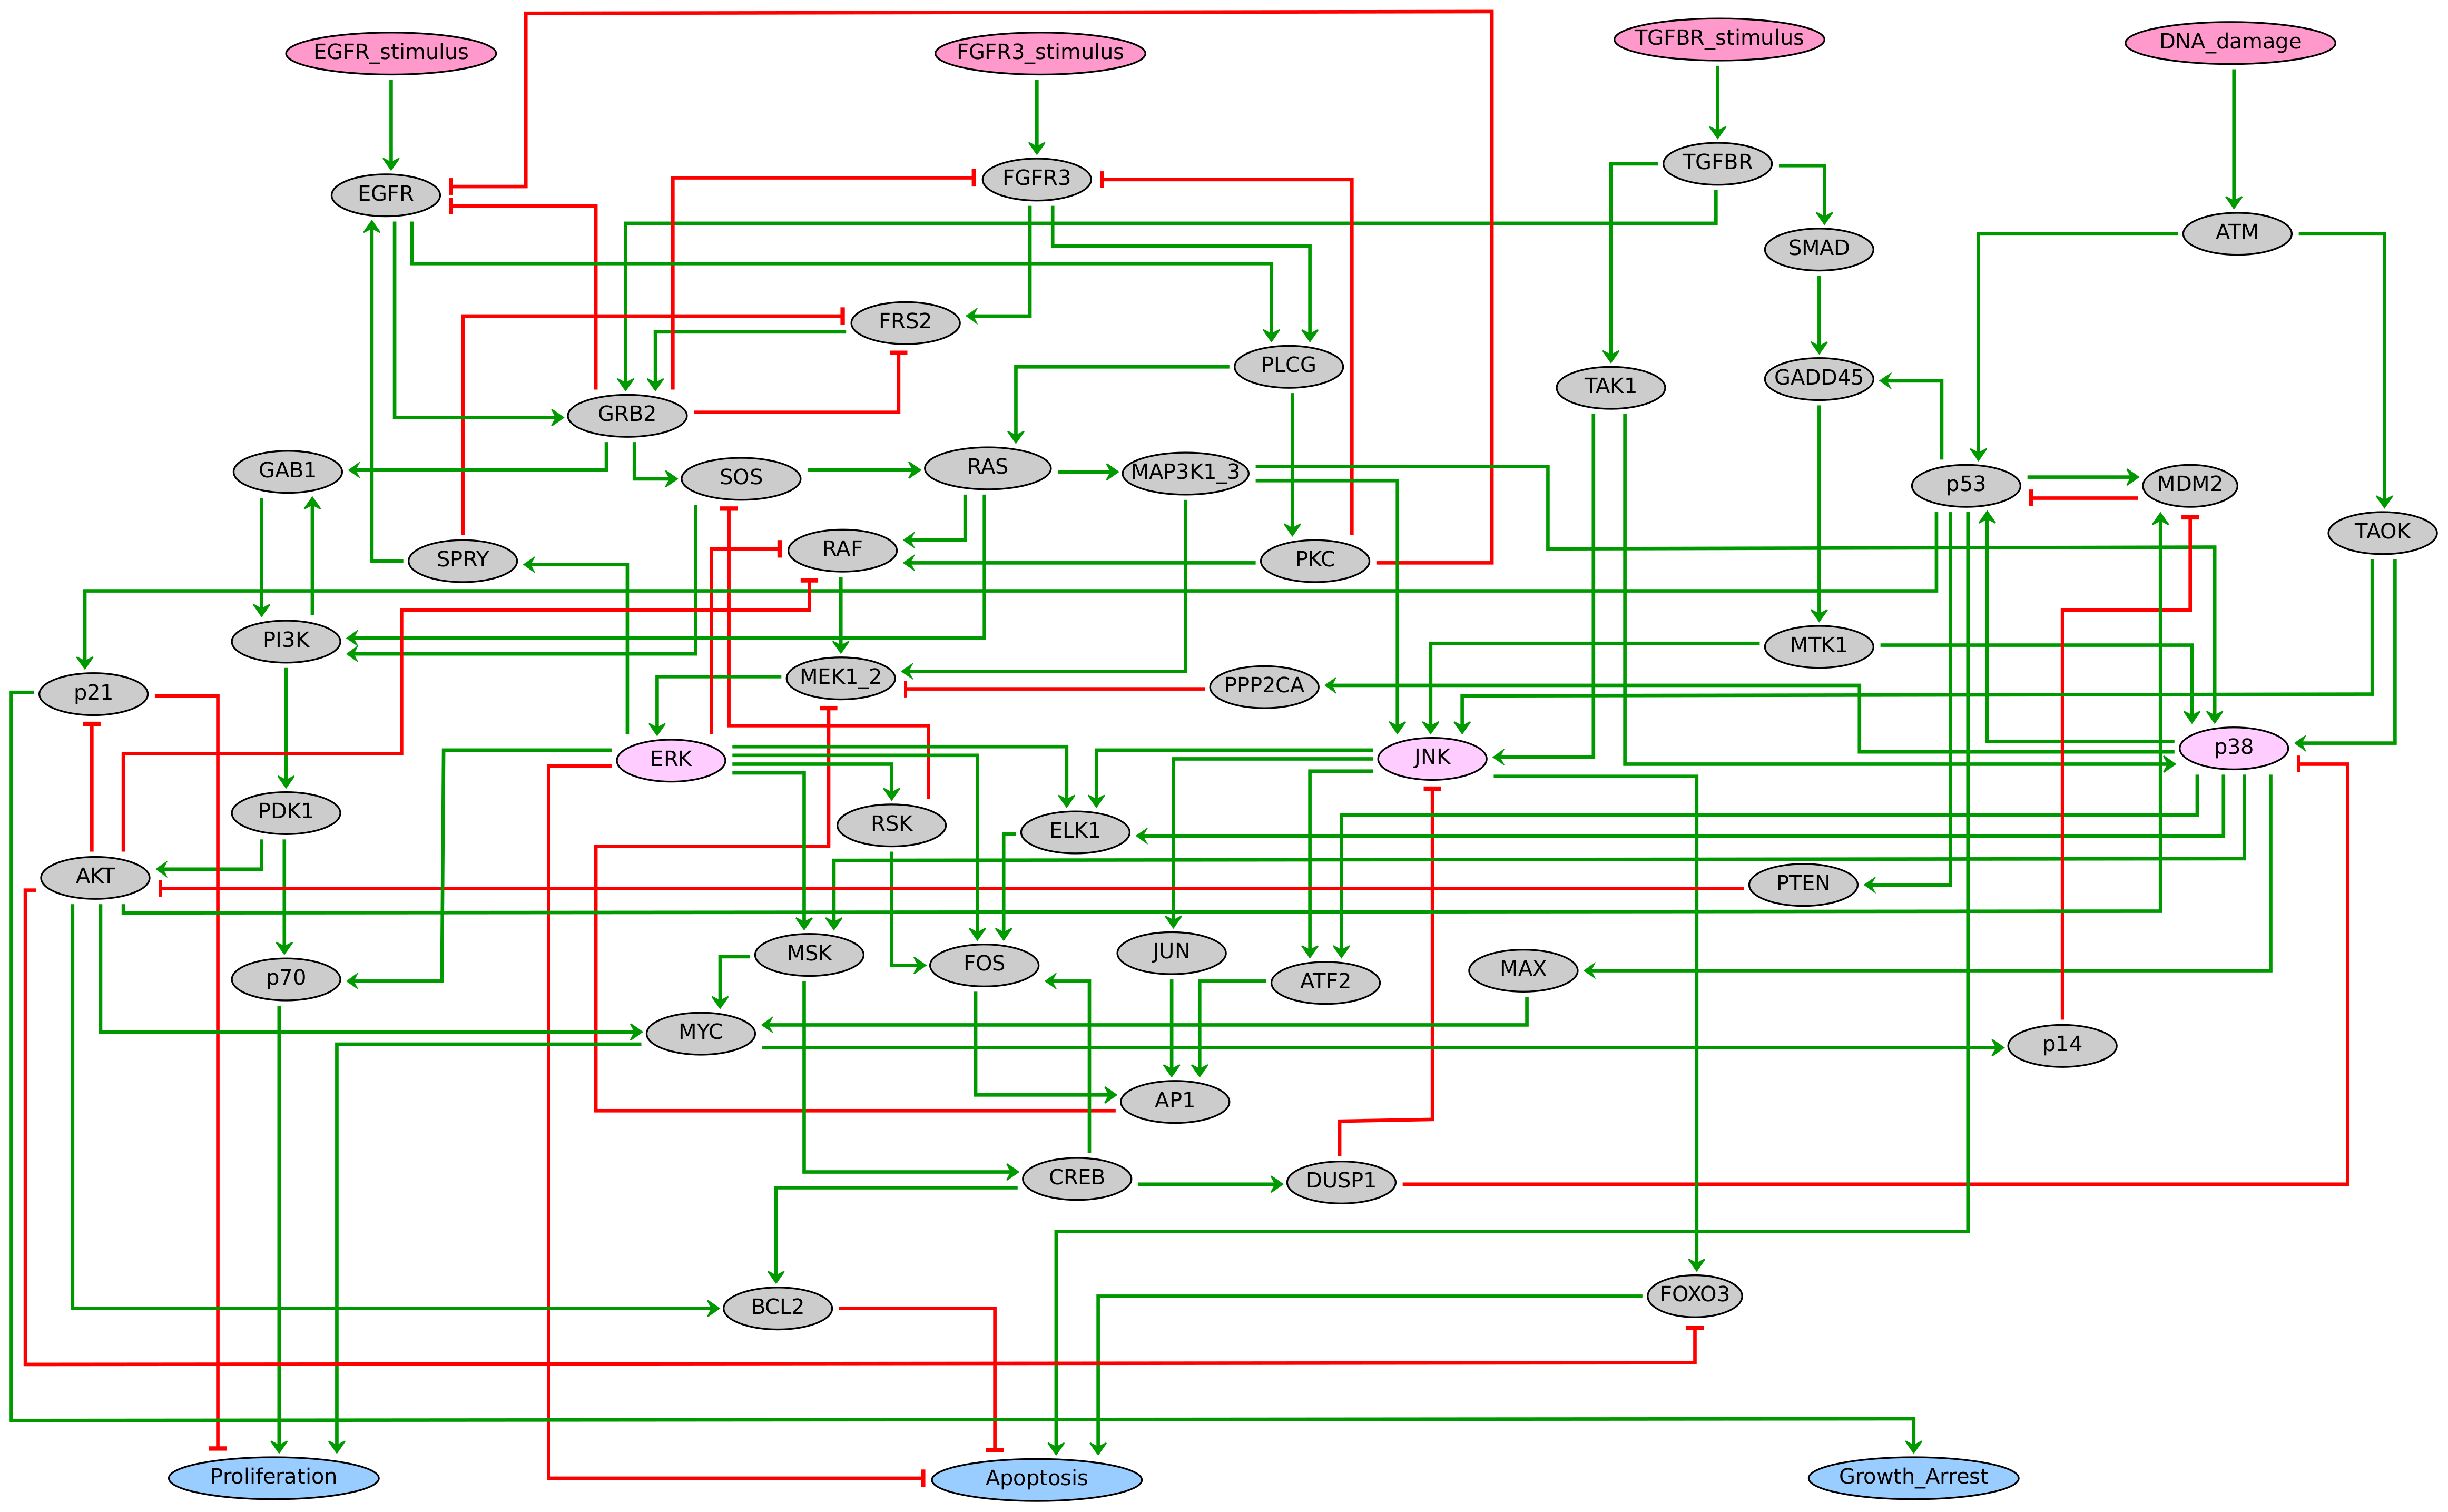
\includegraphics[width=\textwidth]{Figures/grieco_rg.png}
  \caption{\textbf{Regulatory network of the MAPK signalling pathway model.} The model consists of 53 variables and 104 regulatory interactions. The model is directly taken from~\cite{Grieco2013}}
  \label{fig:grieco_rn}
  \end{minipage}
}\end{figure}

% - Model introduction
% - Attractor (phenotype) classification
% - 0000 - control everything
%     - Former Grieco replication
% - ERK vs. (→) phenotypes ?

Another model we consider is the Grieco et al. version of MAPK model as presented in~\cite{Grieco2013}. This model represents a bladder cancer behavior using a combination of three pathways (FGFR3, EFGR, and TGFBR). The model has four inputs (a stimulus for each pathway and a DNA damage). We consider these inputs set to a constant false with an exception to FGFR3 which set to true (as in the previous model).

The regulatory network of the model can be found in \autoref{fig:grieco_rn}. The exact function definitions can be found in \autoref{appendix:digi_attach}.



% \begin{table}[]
% \checkoddpage
% \edef\side{\ifoddpage l\else r\fi}
% \makebox[\textwidth][\side]{% 
% \begin{minipage}[t]{\fullwidth}
% \scriptsize
% \caption{\textbf{Update functions of the isolated FGFR3 pathway modexl.} The table shows the update functions of the variables in the model as in~\cite{Grieco2013}. The variables are ordered alphabetically. The last four variables are inputs of the model.}
% \begin{tabular}{lp{15cm}}
% \hline
% \textbf{Variable} & \textbf{Function} \\
% \hline
% \var{AKT} & \var{PDK1} $\land$ \var{PTEN} \\
% \var{AP1} & \var{JUN} $\land$ (\var{ATF2} $\lor$ \var{FOS}) \\
% \var{ATF2} & \var{JNK} $\lor$ \var{p38} \\
% \var{ATM} & \var{DNA\_damage} \\
% \var{Apoptosis} & (\var{FOXO3} $\land$ \var{p53}) $\land$ $\neg$(\var{BCL2} $\lor$ \var{ERK}) \\
% \var{BCL2} & \var{CREB} $\land$ \var{AKT} \\
% \var{CREB} & \var{MSK} \\
% \var{DUSP1} & \var{CREB} \\
% \var{EGFR} & (\var{EGFR\_stimulus} $\land$ $\neg$(\var{PKC} $\lor$ \var{GRB2})) $\lor$ (\var{SPRY} $\land$ $\neg$(\var{PKC} $\lor$ \var{GRB2})) \\
% \var{ELK1} & (\var{JNK} $\lor$ \var{ERK}) $\lor$ \var{p38} \\
% \var{ERK} & \var{MEK1\_2} \\
% \var{FGFR3} & \var{FGFR3\_stimulus} $\land$ $\neg$(\var{PKC} $\lor$ \var{GRB2}) \\
% \var{FOS} & \var{ERK} $\land$ \var{RSK} $\land$ (\var{CREB} $\lor$ \var{ELK1}) \\
% \var{FOXO3} & \var{JNK} $\land$ $\neg$\var{AKT} \\
% \var{FRS2} & \var{FGFR3} $\land$ $\neg$(\var{GRB2} $\lor$ \var{SPRY}) \\
% \var{GAB1} & \var{PI3K} $\lor$ \var{GRB2} \\
% \var{GADD45} & \var{p53} $\lor$ \var{SMAD} \\
% \var{GRB2} & \var{EGFR} $\lor$ \var{TGFBR} $\lor$ \var{FRS2} \\
% \var{Growth\_Arrest} & \var{p21} \\
% \var{JNK} & (\var{TAOK} $\land$ \var{MAP3K1\_3}) $\lor$ (\var{TAK1} $\land$ $\neg$\var{DUSP1}) $\lor$ (\var{MAP3K1\_3} $\land$ \var{MTK1}) $\lor$ (\var{TAK1} $\land$ \var{MAP3K1\_3}) $\lor$ (\var{MAP3K1\_3} $\land$ $\neg$\var{DUSP1}) $\lor$ (\var{TAK1} $\land$ \var{v\_MTK1}) $\lor$ (\var{TAK1} $\land$ \var{TAOK}) $\lor$ (\var{TAOK} $\land$ \var{MTK1}) $\lor$ (\var{MTK1} $\land$ $\neg$\var{DUSP1}) $\lor$ (\var{TAOK} $\land$ $\neg$\var{DUSP1}) \\
% \var{JUN} & \var{JNK} \\
% \var{MAP3K1\_3} & \var{RAS} \\
% \var{MAX} & \var{p38} \\
% \var{MDM2} & (\var{AKT} $\land$ $\neg$\var{p14}) $\lor$ (\var{p53} $\land$ $\neg$\var{p14}) \\
% \var{MEK1\_2} & (\var{RAF} $\land$ $\neg$(\var{PPP2CA} $\lor$ \var{AP1})) $\lor$ (\var{MAP3K1\_3} $\land$ $\neg$(\var{PPP2CA} $\lor$ \var{AP1})) \\
% \var{MSK} & \var{p38} $\lor$ \var{ERK} \\
% \var{MTK1} & \var{GADD45} \\
% \var{MYC} & (\var{MSK} $\land$ \var{AKT}) $\lor$ (\var{MSK} $\land$ \var{MAX}) \\
% \var{PDK1} & \var{PI3K} \\
% \var{PI3K} & \var{GAB1} $\lor$ (\var{RAS} $\land$ \var{SOS}) \\
% \var{PKC} & \var{PLCG} \\
% \var{PLCG} & \var{EGFR} $\lor$ \var{FGFR3} \\
% \var{PPP2CA} & \var{p38} \\
% \var{PTEN} & \var{p53} \\
% \var{Proliferation} & \var{p70} $\land$ \var{MYC} $\land$ $\neg$\var{p21} \\
% \var{RAF} & (\var{PKC} $\land$ $\neg$(\var{ERK} $\lor$ \var{AKT})) $\lor$ (\var{RAS} $\land$ $\neg$(\var{ERK} $\lor$ \var{AKT})) \\
% \var{RAS} & \var{SOS} $\lor$ \var{PLCG} \\
% \var{RSK} & \var{ERK} \\
% \var{SMAD} & \var{TGFBR} \\
% \var{SOS} & \var{GRB2} $\land$ $\neg$\var{RSK} \\
% \var{SPRY} & \var{ERK} \\
% \var{TAK1} & \var{TGFBR} \\
% \var{TAOK} & \var{ATM} \\
% \var{TGFBR} & \var{TGFBR\_stimulus} \\
% \var{p14} & \var{MYC} \\
% \var{p21} & \var{p53} $\land$ $\neg$\var{AKT} \\
% \var{p38} & (\var{MAP3K1\_3} $\land$ \var{MTK1}) $\lor$ (\var{TAK1} $\land$ $\neg$\var{DUSP1}) $\lor$ (\var{TAOK} $\land$ \var{MAP3K1\_3}) $\lor$ (\var{MAP3K1\_3} $\land$ $\neg$\var{DUSP1}) $\lor$ (\var{TAK1} $\land$ \var{MAP3K1\_3}) $\lor$ (\var{TAOK} $\land$ $\neg$\var{DUSP1}) $\lor$ (\var{TAK1} $\land$ \var{MTK1}) $\lor$ (\var{TAK1} $\land$ \var{TAOK}) $\lor$ (\var{MTK1} $\land$ $\neg$\var{DUSP1}) $\lor$ (\var{TAOK} $\land$ \var{MTK1}) \\
% \var{p53} & (\var{p38} $\land$ $\neg$\var{MDM2}) $\lor$ (\var{ATM} $\land$ $\neg$\var{MDM2}) $\lor$ (\var{ATM} $\land$ \var{p38}) \\
% \var{p70} & \var{PDK1} $\land$ \var{ERK} \\
% \var{DNA\_damage} & \var{FALSE} \\
% \var{EGFR\_stimulus} & \var{FALSE} \\
% \var{FGFR3\_stimulus} & \var{TRUE} \\
% \var{TGFBR\_stimulus} & \var{FALSE} \\
% \hline
% \end{tabular}
% \label{tab:grieco_funs}
% \end{minipage}
% }
% \end{table}



Moreover, the MAPK model contains three outputs variables (apoptosis, growth arrest, proliferation). These outputs are then used to represent the four cardinal phenotypes of the model. These phenotypes and their exact configuration is depicted in \autoref{tab:grieco_phenotypes}.


\begin{table}[ht!]
  \checkoddpage
  \edef\side{\ifoddpage l\else r\fi}
  \makebox[\textwidth][\side]{% 
	\begin{minipage}[t]{\fullwidth}
  \small
  \caption{\textbf{MAPK phenotypes.} The cardinal phenotypes of the Grieco MAPK model which will be used throughout the experiments. The first two columns represent the full name and abbreviation of the phenotype. The last three columns represent the model output values which are representing a given phenotype.} 
  \centering
  \begin{tabular}{lc|ccc}
  \hline 
  \textbf{Phenotype} & \textbf{Abbreviation} & \textbf{Apoptosis} & \textbf{Growth arrest} & \textbf{Proliferation} \\
  \hline
  Apoptosis     & A & 1         & *             & 0             \\
  Growth arrest & GA & 0         & 1             & 0             \\
  Proliferation & P & 0         & 0             & 1             \\
  No decision   & ND & 0         & 0             & 0          \\
  \hline  \addlinespace
  \end{tabular}
  \label{tab:grieco_phenotypes}
  \end{minipage}
  }
\end{table}

\begin{table}[!htbp]
  \checkoddpage
  \edef\side{\ifoddpage l\else r\fi}
  \makebox[\textwidth][\side]{% 
	\begin{minipage}[t]{\fullwidth}
  \caption{\textbf{MAPK perturbations.} A list of perturbations of size up to 1 which drive the MAPK model to a phenotype given in the first column. An $\emptyset$ symbol stands for no perturbation while perturbations contained in the square brackets are needed to be combined in order to achieve the perturbation goal. The last column contains a count of unique smallest perturbations achieving the given phenotype.}
  \centering
  \begin{tabular}{lll}
  \textbf{Phenotype} & \textbf{Perturbations} & \textbf{\#}\\ \midrule
  Apoptosis & \begin{tabular}[c]{@{}l@{}}\blue{\var{ATM}=1; \var{CREB}=0; \var{DNA\_damage}=1; \var{DUSP1}=0; \var{FRS2}=1;} \blue{\var{GRB2}=1; \var{TAK1}=1;} \\ \blue{\var{TAOK}=1; \var{TGFBR}=1; \var{TGFBR\_st.}=1}\end{tabular} & 10 \\  [2ex]
  Growth arrest & \begin{tabular}[c]{@{}l@{}} [\var{AKT}=\var{p21}=1]; \blue{[\var{ATM}=\var{BCL2}=1]}; \blue{[\var{ATM}=\var{ERK}=1]}; \blue{$[$\var{ATM}=1,\var{FOXO3}=0]}; ... \end{tabular} & 85 \\ 
  No decision & \begin{tabular}[c]{@{}l@{}}\var{FGFR3}=0; \var{FGFR3\_st.}=0; \var{MAP3K1\_3}=0; \var{MSK}=0; \var{MYC}=0; \var{PKC}=1; \var{RAS}=0\end{tabular} & 7 \\ 
  Proliferation & \blue{\var{ERK}=1}; \var{MEK1\_2}=1; \var{RAF}=1 & 3\\ \midrule
  \begin{tabular}[c]{@{}l@{}}\oscil A-GA \end{tabular} & \var{p21}=1, \var{p38}=1, \var{p53}=1 & 3 \\ [1ex]
  \oscil A-ND & \begin{tabular}[c]{@{}l@{}} [\var{AP1}=1,\var{p21}=0]; [\var{ERK}=\var{p21}=0]; [\var{GRB2}=\var{p21}=0]; $[$\var{JNK}=1,\var{p21}=1]; ...\end{tabular} & 10 \\
  \oscil A-P & N/A & 0 \\ [1ex]
  \begin{tabular}[c]{@{}l@{}}\oscil GA-ND \end{tabular} & \begin{tabular}[c]{@{}l@{}} \blue{[\var{AP1}=\var{BCL2}=1]; [\var{AP1}=1,\var{FOXO3}=0]}; [\var{AP1}=1=\var{JNK}=0]; \blue{$[$\var{BCL2}=1,\var{ERK}=0]}; ... \end{tabular} & 26 \\
  \begin{tabular}[c]{@{}l@{}}\oscil GA-P \end{tabular} & N/A & 0 \\ [2ex]
  \begin{tabular}[c]{@{}l@{}}\oscil ND-P \end{tabular} & \begin{tabular}[c]{@{}l@{}} \var{AKT}=1; \var{CREB}=1; \var{DUSP1}=1; \var{MDM2}=1; \var{MSK}=1; \var{PTEN}=0; \var{p14}=0; \var{p21}=0; \\ \var{p38}=0; \blue{\var{p53}=0} \end{tabular} & 10 \\ \midrule
  \begin{tabular}[c]{@{}l@{}}\oscil A-GA-ND \end{tabular} & \begin{tabular}[c]{@{}l@{}} \var{AP1}=1; \var{ERK}=0; \var{GRB2}=0; \var{JNK}=1; \var{MEK1\_2}=0; \var{PDK1}=0; \var{PI3K}=0; \var{PPP2CA}=1;\\ \var{p70}=0 \end{tabular} & 9 \\ [2ex]
  \begin{tabular}[c]{@{}l@{}}\oscil A-GA-P \end{tabular} & N/A & 0 \\ [1ex]
  \begin{tabular}[c]{@{}l@{}}\oscil A-ND-P \end{tabular} & \begin{tabular}[c]{@{}l@{}} \var{p21}=0 \end{tabular} & 1 \\ [1ex]
  \begin{tabular}[c]{@{}l@{}}\oscil GA-ND-P \end{tabular} & \blue{\var{BCL2}=1}; \blue{\var{FOXO3}=0}; \var{JNK}=0 & 3 \\ \midrule
  \begin{tabular}[c]{@{}l@{}}\oscil $\forall$ \end{tabular} & $\emptyset$ & 1  \\ 
  \midrule
  \end{tabular}
      \label{tab:grieco_phenotypes_perturbations}
  \end{minipage}
  }
\end{table}

In the study~\cite{Grieco2013}, the full model version with 53 variables was presented. However, the simulations of knockout and over-expression experiments were performed on a reduced variant of the model (having only 17 variables) to observe how they impact the model phenotypes. Our novel approach allows us to consider the full model and all possible perturbations of the model at once, which helps us to obtain more comprehensive results. \autoref{tab:grieco_phenotypes_perturbations} shows the exhaustive enumeration of one-size perturbations which lead to any phenotype (as in \autoref{tab:grieco_phenotypes}), including all observed combinations of phenotype oscillations.


Stabilization in all phenotypes apart from growth arrest is possible with perturbations of size one. The unperturbed model behavior is an oscillation through all phenotypes. Moreover, disabling the only input set to true, \var{FGFR3\_stimulus}, causes the model to stabilize in the no-decision phenotype.

The results also highlight the influence of ERK, which represented the phenotype in the previous model. Since perturbing ERK leads to proliferation, ERK appears to be a strong driver of the proliferation phenotype. However, several previously observed drivers stabilizing ERK (from \autoref{sec:mapk_case_study_isolated}) are not present among the perturbations of the full model. This may be because the full model contains more variables, making their influence on ERK more complex.

% Last but not least, we can observe that the model as proposed in~\cite{Grieco2013} exhibits oscillations in numerous combinations of phenotypes under relatively small perturbations. Specifically, there are decisions containing oscillation between apoptosis and other phenotype. Such a behavior is difficult to interpret since a real-world system would be expected to continue in proliferation after committing to conduct the apoptosis. 

\subsection{Extended FGFR3 pathway MAPK}

To demonstrate our method on a larger-scale model, we extend the fully specified model~\cite{Grieco2013} that puts FGFR3-MAPK signalling into a broader context of protein interactions having the crucial impact on cell growth. The model has originally targeted bladder tissue cells. Our extension employs the PSBN framework allowing us to establish a partially specified model that incorporates mechanisms which are not yet understood well. In particular, based on Reactome~\cite{Milacic2023} and state-of-the-art knowledge~\cite{Fafilek2018,Fafilek2022} we compile an extended model bringing the updated FGFR3 activation mechanism to the Grieco model. 


\begin{table}[htbp!]
\checkoddpage
\edef\side{\ifoddpage l\else r\fi}
\makebox[\textwidth][\side]{% 
\begin{minipage}[t]{\fullwidth}
\caption{\textbf{Changes done to model MAPK model.} The table shows the changes done to the original model~\cite{Grieco2013} in order to obtain the extended model. The first column shows the variable and a type of the change. The second column shows the original list of regulations or functions. The third column shows the new list of regulations or functions with the changes highlighted in \textcolor{blue}{blue} font. The regulations marked with + are positives, - are negatives and ? denotes that regulation might not be present in an interpretation. Double ?? denotes that the regulation might be present in an interpretation as both positive and negative. Functions are denoted with $f$ and $g$ are the functions which are not specified in the model, but their instance must adhere to the listed regulations.}
\begin{tabular}{lll}
\hline
 &  \textbf{Original} & \textbf{New} \\
\hline
\var{FGFR3} reg. & \var{FGFR3\_stim}+, \var{GRB2}-, \var{PKC}- & \var{FGFR3\_stim}+, \var{GRB2}-\textcolor{blue}{?}, \var{PKC}-\textcolor{blue}{?} \\
 \var{FGFR3} def. & \var{FGFR3\_stim} $\land$ $\neg$(\var{GRB2} $\lor$ \var{PKC}) & \var{FGFR3\_stim} $\land$ \textcolor{blue}{$f$(\var{GRB2},\var{PKC})} \\
\var{FRS2} reg. & \var{FGFR3}+, \var{GRB2}-, \var{SPRY}- & \textcolor{blue}{\var{ERK}-?}, \var{FGFR3}+, \var{GRB2}-\textcolor{blue}{?}, \textcolor{blue}{\var{SHIP2}??}, \var{SPRY}-\textcolor{blue}{?} \\
\var{FRS2} def. & \var{FGFR3} $\land$ $\neg$(
\var{GRB2} $\lor$ \var{SPRY}) & \textcolor{blue}{$g$(\var{FGFR3},\var{ERK},\var{GRB2},\var{SHIP2},\var{SPRY})} \\
\hline
\end{tabular}
\label{tab:grieco_extension}
\end{minipage}
}
\end{table}

\begin{table}[htbp!]
\checkoddpage
\edef\side{\ifoddpage l\else r\fi}
\makebox[\textwidth][\side]{% 
\begin{minipage}[t]{\fullwidth}
\centering
\caption{\textbf{Extended MAPK model performance.} The table shows the performance of the extended MAPK model. The first column shows the phenotype, the second column shows the relation to the perturbation (standard, avoid, oscillation), and the third column shows the time of the computation. The computations were performed on a computer with AMD Ryzen Threadripper 2990WX 32-Core Processor and 64GB of memory.}
\begin{tabular}{llr}
\phenotype & \textbf{relation} & \multicolumn{1}{l}{\textbf{time}} \\
\hline
GA & standard & 00:02:45 \\
P & standard & 00:24:59 \\
A & standard & 00:35:59 \\
A & avoid & 00:39:26 \\
ND & avoid & 00:40:00 \\
GA & avoid & 00:41:56 \\
ND & standard & 01:13:09 \\
GA & oscillation & 01:17:13 \\
A & oscillation & 02:42:08 \\
P & avoid & 03:50:26 \\
ND & oscillation & 04:05:15 \\
P & oscillation & 13:09:52 \\
\hline
\end{tabular}
\label{tab:fgfr3extended_perf}
\end{minipage}
}
\end{table}




This is done by embedding the isolated FGFR3-MAPK pathway studied in previous section. At the level of regulations, the embedding brings in: 

\begin{enumerate}
  \item Addition of SHIP2 affecting the FRS2 adapter phoshorylation capabilities as discussed within the isolated model
  \item Addition of the positive feedback from ERK to FRS2 (experimentally studied mostly in the context of chondrocytes)
  \item Addition of the positive feedback from ERK to GRB2 (experimentally studied mostly in the context of chondrocytes)
\end{enumerate}

At the level of logical rules, the update functions of \var{FGFR3} and \var{FRS2} are made unspecified with the only constraint that \var{FGFR3\_stimulus} is left as a necessary precursor of \var{FGFR3} activation. The chosen level of abstraction reflects the fact that biochemical mechanisms specifying how the respective regulations affecting \var{FGFR3} and \var{FRS2} are combined are not currently known. Same as before, we consider the inputs to be fixed to 0, with an exception to FGFR3 stimulus. The resulting model contains 54 variables and four cardinal phenotypes as described in~\cite{Grieco2013} -- apoptosis (A), growth arrest (GA), no decision (ND), and proliferation (P). The exact overview of the model changes is available in the \autoref{tab:grieco_extension}.


\begin{figure}[htbp!]
  \centering
  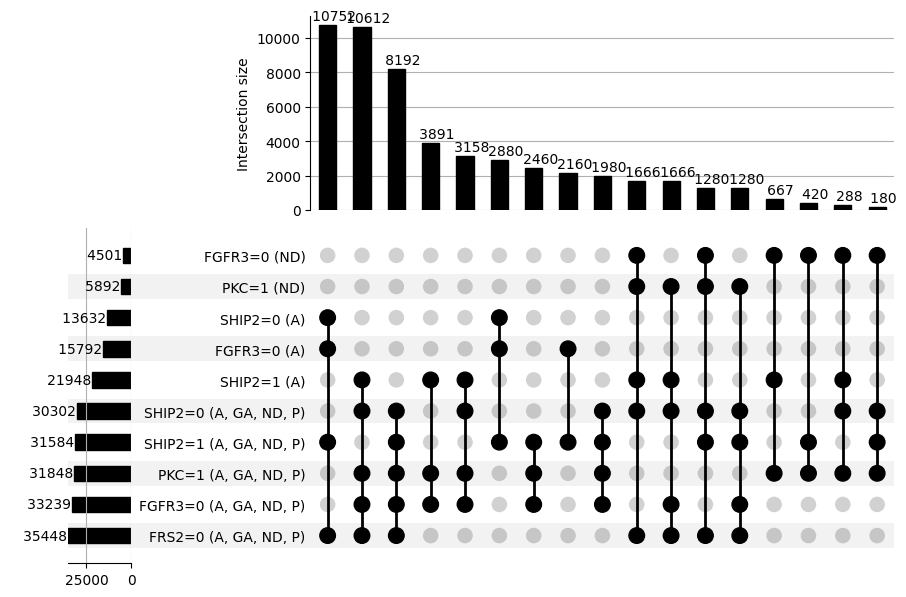
\includegraphics[width=\textwidth]{Figures/upset_extended.png}
  \caption{\textbf{Upset plot for the FGFR3 extended model.} The plot clearly shows, that each perturbation achieves a unique interpretation partitioning. Moreover, it is not possible to achieve two different phenotypes at once using the same perturbation. The perturbations are not unique, since we consider all phenotypes and perturbations at once.}
  \label{fig:extended_upset}
\end{figure}


The goal of the analysis is to apply control-guided refinement to identify perturbations that can reduce the set of possible interpretations of the extended PSBN. We consider the hypotheses on the FGFR3 signalling mechanisms stated in previous section and the pior knowledge based on~\cite{Grieco2013,Vaque2014,Stanislaus2012}.



First, we compute control for all phenotypes including oscillations among them. We restrict the results to perturbations of size up to 1. The performance results are shown in \autoref{tab:fgfr3extended_perf}. We can see, that our method was able to compute perturbations for all cardinal phenotypes in a reasonable time.

\sethlcolor{green!30}
\begin{table}[btph!]
  \caption{\textbf{Phenotype control of extended MAPK model.} The first column shows the (stable) phenotype or multiple oscillating phenotypes manifested by the model under perturbations listed in the second column. Perturbations in \textcolor{blue}{blue} font are working in the original~\cite{Grieco2013} model. Perturbations highlighted in \hl{green} are the reference perturbations we used for the model refinement. The third column displays the long-term ERK activity, and the last column shows the robustness of respective perturbations. The symbol '*' denotes that we observe amiguous ERK behavior under the given perturbations.}
  \centering
  \small
  \begin{tabular}{rlccc}
  \textbf{\phenotype} & \textbf{Perturbations} & ERK & $\robustness$ for $\allInterpretations$ & $\robustness$ for $\interpretationSet$ \\ \midrule
  A & \begin{tabular}[c]{@{}l@{}}\textcolor{blue}{\var{ATM}=1,\var{CREB}=0,\var{DNA\_dmg}=1,\var{DUSP1}=0},\\ \textcolor{blue}{\var{TAK1}=1,\var{TAOK}=1,\var{TGFBR}=1,\var{TGFBR\_st.}=1}\end{tabular} & 0 & 1 & 1\\
  & \varhl{PLCG}\hl{=0} & 0 & 0.80 & 1\\ 
  & \textcolor{blue}{\var{FRS2}=1,\var{GRB2}=1} & 0 & 0.64 & 1\\
  & \begin{tabular}[c]{@{}l@{}}\var{AP1}=1,\var{ERK}=0,\var{GADD45}=1,\var{JNK}=1,\var{JUN}=1,\\\var{MEK1\_2}=0,\var{MTK1}=1,\var{PPP2CA}=1,\var{SMAD}=1,\\ \var{p38}=1,\var{p53}=1,\var{SHIP2}=1,\var{SHIP2}=0,\var{PKC}=1,\\\O,\var{SPRY},\var{RSK}=0,\var{PKC}=0,\var{SPRY}=1 \end{tabular} & 0 & $<$0.6 & $<$0.5\\
  \midrule
  GA & \var{BCL2}=1,\var{FOXO3}=0,\var{JNK}=0 & 0 & 0.61 & 0 \\ 
  & \var{ERK}=1,\var{MEK1\_2}=0,\var{p21}=1 & 1 & $<$0.3 & 0 \\ 
  \midrule
  ND & \begin{tabular}[c]{@{}l@{}}\var{AKT}=1,\var{PTEN}=0;\var{p38}=0\end{tabular} & 0 & 0.61 & 0 \\ 
  & \begin{tabular}[c]{@{}l@{}}\textcolor{blue}{\var{MAP3K1\_3}=0,\var{MSK}=0,\var{MYC}=0,\var{RAS}=0} \end{tabular} & * & 0.50 & 1 \\ 
  & \begin{tabular}[c]{@{}l@{}}\var{AKT}=0,\textcolor{blue}{\var{FGFR3}=0},\var{GAB1}=0,\var{RSK}=1,\var{SOS}=0, \\ \textcolor{blue}{\var{FGFR3\_stimulus}=0},\var{p53}=0,\var{p70}=0, \\ \var{PDK1}=0,\var{PI3K}=0,\textcolor{blue}{\var{PKC}=1},\var{PLCG}=0,\var{PTEN}=1\end{tabular} & * & $<$0.3 & $<$0.2 \\ 
  \midrule
  P & \textcolor{blue}{\varhl{ERK}\hl{=1}, \var{MEK1\_2}=1} & 1 & 0.3 & 1 \\ 
  & \textcolor{blue}{\var{RAF}=1} & 1 & 0.19 & 1 \\ 
  & \begin{tabular}[c]{@{}l@{}}\var{GAB1}=1,\var{GADD45}=0,\var{MAX}=0,\var{MDM2}=1, \\ \var{MTK1}=0,\var{p14}=0,\var{p53}=0,\var{PDK1}=1,\var{PI3K}=1
  \end{tabular} & 1 & $<$0.1 & 0 \\
  \midrule

  A-GA & \textcolor{blue}{\var{p38}=1,\var{p53}=1} & 0 & 0.25 & 1 \\
  & \textcolor{blue}{\var{p21}=1} & * & 0.19 & 1 \\  

  ND-P & \begin{tabular}[c]{@{}l@{}} \textcolor{blue}{\var{p53}=0} \end{tabular} & \oscil & 0.55 & 1 \\ 
  & \begin{tabular}[c]{@{}l@{}} \textcolor{blue}{\var{MDM2}=1,\var{p14}=0},\textcolor{blue}{\var{AKT}=1,\var{CREB}=1,\var{DUSP1}=1,} \\ \textcolor{blue}{\var{MSK}=1,\var{PTEN}=0,\var{p38}=0} \end{tabular} & \oscil & $<$0.3 & 1 \\ 

  A-GA-ND & \begin{tabular}[c]{@{}l@{}} \textcolor{blue}{\var{AP1}=1,\var{ERK}=0,\var{JNK}=1,\var{MEK1\_2}=0,}\textcolor{blue}{\var{PPP2CA}=1}\end{tabular} & 0 & 0.25 & 1 \\ 
  & \begin{tabular}[c]{@{}l@{}}\textcolor{blue}{\var{GRB2}=0}\end{tabular} & \oscil & 0.2 & 0.6 \\   
  & \begin{tabular}[c]{@{}l@{}}\textcolor{blue}{\var{PDK1}=0, \var{PI3K}=0, \var{p70}=0}\end{tabular} & \oscil & $<$0.2 & 1 \\   


  A-ND-P & \begin{tabular}[c]{@{}l@{}} \textcolor{blue}{\var{p21}=0} \end{tabular} & \oscil & 0.19 & 1 \\  

  GA-ND-P & \textcolor{blue}{\var{BCL2}=1; \var{FOXO3}=0; \var{JNK}=0} & \oscil & 0.19 & 1 \\ \midrule
  \oscil $\forall$
  & \textcolor{blue}{\hl{\O}} & \oscil & 0.28 & 1 \\  
  \midrule
  \end{tabular}
  \label{tab:fgfr3extended}
\end{table}

\begin{table}[htb!]
  \caption{\textbf{Behavior of interpretations under perturbations of extended MAPK model.} The first column denotes the size of the interpretation set, while the next five columns denote the behavior of the interpretations under the selected perturbations. The $\mid$ separates possible bi-stability outcome while $\oscil$ denotes oscillation between all model phenotypes.}
\centering
  \begin{tabular}{r|ccccc}
  $\mid \interpretationSet \mid$ & \var{FGFR3}=0 & \var{FRS2}=0 & \var{PKC}=1 & \var{SHIP2}=0 & \var{SHIP2}=1 \\  \hline
  10752 & A        & $\oscil$         & A        & A             & $\oscil$         \\
  10612 & $\oscil$ & $\oscil$         & $\oscil$ & $\oscil$      & A                \\
  8192  & $\oscil$ & $\oscil$         & $\oscil$ & $\oscil$      & $\oscil$         \\
  3848  & $\oscil$ & A$\mid$ND$\mid$P & $\oscil$ & ND$\mid$P     & A                \\
  3158  & $\oscil$ & A$\mid$ND$\mid$P & $\oscil$ & $\oscil$      & A                \\
  2880  & A        & A$\mid$ND$\mid$P & A        & A             & $\oscil$         \\
  2430  & $\oscil$ & A$\mid$ND$\mid$P & $\oscil$ & ND$\mid$P     & $\oscil$         \\
  2160  & A        & A$\mid$ND$\mid$P & A        & A$\mid$ND$\mid$P & $\oscil$     \\
  1980  & $\oscil$ & A$\mid$ND$\mid$P & $\oscil$ & $\oscil$      & $\oscil$         \\
  1666  & ND       & $\oscil$         & ND       & $\oscil$      & A                \\
  1666  & $\oscil$ & $\oscil$         & ND       & $\oscil$      & A                \\
  1280  & ND       & $\oscil$         & ND       & $\oscil$      & $\oscil$         \\
  1280  & $\oscil$ & $\oscil$         & ND       & $\oscil$      & $\oscil$         \\
  624   & ND       & A$\mid$ND$\mid$P & $\oscil$ & ND$\mid$P     & A                \\
  390   & ND       & A$\mid$ND$\mid$P & $\oscil$ & ND$\mid$P     & $\oscil$         \\
  288   & ND       & A$\mid$ND$\mid$P & $\oscil$ & $\oscil$      & A                \\
  180   & ND       & A$\mid$ND$\mid$P & $\oscil$ & $\oscil$      & $\oscil$         \\
  43    & ND       & A$\mid$ND$\mid$P & $\oscil$ & A$\mid$ND$\mid$P & A            \\
  43    & $\oscil$ & A$\mid$ND$\mid$P & $\oscil$ & A$\mid$ND$\mid$P & A            \\
  30    & $\oscil$ & A$\mid$ND$\mid$P & $\oscil$ & A$\mid$ND$\mid$P & $\oscil$     \\
  30    & ND       & A$\mid$ND$\mid$P & $\oscil$ & A$\mid$ND$\mid$P & $\oscil$     \\
  \end{tabular}
  \label{tab:fgfr3extended_phenotypes}
  \end{table}

The results are shown in \autoref{tab:fgfr3extended}. We can see, that perturbations can achieve all the four cardinal phenotypes as well as achievable oscillations among them. We can also observe the correlation between the ERK activity and the proliferation phenotype -- in particular, the ERK stabilization is required for the proliferation phenotype, while apoptosis phenotype drives ERK avoidance.

The results highlighted in blue correspond with the perturbations computed on the original model~\cite{Grieco2013} (see \autoref{tab:grieco_phenotypes_perturbations}). Moreover, the results include several perturbations that have not been observed before. Notably, there is the perturbation \var{PLCG}=0 which leads to apoptosis stabilization. This perturbation is not present in the original model, however, it has been observed in~\cite{Vaque2014,Stanislaus2012} that PLCG is a driver for cell proliferation while its inhibition can lead to apoptosis. This is a strong evidence that this perturbation is indeed valid, and we can use it for our model refinement.

Based on the discussion above, the perturbations \var{ERK}=1 (achieving proliferation) and \var{PLCG}=0 (leading to apoptosis) are strongly affecting the long-term behavior of the model. To that end, we use this knowledge to complete the first iteration of the control-guided refinement procedure.



Analogously to the isolated model case study, we compute the new control results shown in the last column of \autoref{tab:fgfr3extended}. 


Next, we select perturbations achieving partitioning to distinct behavior patterns. Due to a big number of viable perturbations with non-100\% robustness, we first cross-compared all combinations of perturbations and phenotypes they achieve, to obtain a set of perturbation equivalence classes. Such equivalence classes were 10 having 1-3 members. Then, we selected one perturbation from each equivalence class. To verify, that they are indeed unique, we show their intersections in \autoref{fig:extended_upset}. Since we consider all phenotypes and perturbations at once, the perturbations are not unique. With upset diagram, we confirmed that all perturbations help with the interpretation classes partitioning unique and, that no perturbation achieves two different phenotypes at once what is expected for the correctness of our method. 


As a result we obtain only five distinct perturbations promising for the model refinement. The perturbations are shown in \autoref{tab:fgfr3extended_phenotypes}. The table displays the admissible perturbations that can be considered for \emph{in vitro} perturbation experiments design leading to potential exclusion of non-complying interpretations of the PSBN. The wet lab testing is necessary to complete the second iteration of the model refinement process, as illustrated in \autoref{fig:control_workflow}. 

\section{Summary}

In this chapter, we have demonstrated the applicability of our method on two case studies. The primary application of control was to make cell reprogramming perturbations. This type of application is commonly used for therapy design, where the goal is to find perturbations that can drive the system from a diseased state to a healthy one. We have shown the application on a myeloid differentiation model, where we have found perturbations that can drive the system between different types of cell differentiations.

Next, we have shown a framework for the model refinement using control. We have applied this framework on a MAPK model variants where we demonstrated how to use the control results to refine the model and reduce the set of possible interpretations either analytically or searching for perturbations that can be used for the wet lab experiments design.